\documentclass[10pt,landscape]{article}
\usepackage{multicol}
\usepackage{calc}
\usepackage{ifthen}
\usepackage{color,soul}
\usepackage{xcolor}
\usepackage{graphicx}
\usepackage[landscape]{geometry}
\usepackage{amsmath}
\usepackage{amssymb}
\usepackage{hyperref}
\DeclareMathOperator{\Tr}{Tr}
% To make this come out properly in landscape mode, do one of the following
% 1.
%  pdflatex latexsheet.tex
%
% 2.
%  latex latexsheet.tex
%  dvips -P pdf  -t landscape latexsheet.dvi
%  ps2pdf latexsheet.ps


% If you're reading this, be prepared for confusion.  Making this was
% a learning experience for me, and it shows.  Much of the placement
% was hacked in; if you make it better, let me know...


% 2008-04
% Changed page margin code to use the geometry package. Also added code for
% conditional page margins, depending on paper size. Thanks to Uwe Ziegenhagen
% for the suggestions.

% 2006-08
% Made changes based on suggestions from Gene Cooperman. <gene at ccs.neu.edu>


% To Do:
% \listoffigures \listoftables
% \setcounter{secnumdepth}{0}


% This sets page margins to .5 inch if using letter paper, and to 1cm
% if using A4 paper. (This probably isn't strictly necessary.)
% If using another size paper, use default 1cm margins.
\ifthenelse{\lengthtest { \paperwidth = 11in}}
	{ \geometry{top=.2in,left=.2in,right=.2in,bottom=.2in} }
	{\ifthenelse{ \lengthtest{ \paperwidth = 297mm}}
		{\geometry{top=0cm,left=0cm,right=0cm,bottom=0cm} }
		{\geometry{top=0cm,left=0cm,right=0cm,bottom=0cm} }
	}

% Turn off header and footer
\pagestyle{empty}
 

% Redefine section commands to use less space
\makeatletter
\renewcommand{\section}{\@startsection{section}{1}{0mm}%
                                {-1ex plus -.5ex minus -.2ex}%
                                {0.5ex plus .2ex}%x
                                {\normalfont\large\bfseries}}
\renewcommand{\subsection}{\@startsection{subsection}{2}{0mm}%
                                {-1explus -.5ex minus -.2ex}%
                                {0.5ex plus .2ex}%
                                {\normalfont\normalsize\bfseries}}
\renewcommand{\subsubsection}{\@startsection{subsubsection}{3}{0mm}%
                                {-1ex plus -.5ex minus -.2ex}%
                                {1ex plus .2ex}%
                                {\normalfont\small\bfseries}}
\makeatother

% Define BibTeX command
\def\BibTeX{{\rm B\kern-.05em{\sc i\kern-.025em b}\kern-.08em
    T\kern-.1667em\lower.7ex\hbox{E}\kern-.125emX}}

% Don't print section numbers
\setcounter{secnumdepth}{0}


\setlength{\parindent}{0pt}
\setlength{\parskip}{0pt plus 0.5ex}


% -----------------------------------------------------------------------

\begin{document}
\footnotesize
\begin{multicols*}{3}
\hl{\textbf{Introduction}}\\
\fbox{\begin{minipage}{\linewidth}
- quintessential example of a representation learning algorithm is the \textbf{auto-encoder}. An auto-encoder is the combination of an encoder function, which converts the input data into a diffeernt representation, and a decoder function, which converts the new representation back into the oirginal format.\newline
- \textbf{factor of variation}: separate sources of influence. In speech analysis, e.g. speaker's age, sex, accent, words they are speaking.\newline 
- quintessential example of deep learning model is the \textbf{feedforward network or multi-layer perceptron (MLP)}. A MLP is just a mathematical function mapping some set of input values to output values.
\end{minipage}}
\hl{\textbf{Linear Algebra}}\\
tensor = array with more than two axes \newline
element-wise or Hadamard product, denoted as $\mathbf{A} \circ \mathbf{B}$ \newline
\fbox{\begin{minipage}{\linewidth}
\textbf{Determinant:} \\
maps matrices to real scalars \\
determinant = product of all eigenvalues \\
abs(det(A)) = a measure of how much multiplication by the matrix expands or contracts space
\end{minipage}}
\hl{\textbf{Probability and Information Theory}}\\
Marginal probability (Sum rule):\\
\fbox{\begin{minipage}{\linewidth}
$P(\text{x}=x) = \sum_y P(\text{x}=x,\text{y}=y)$, or
$p(x) =\int p(x,y)dy$
\end{minipage}}
Conditional probability \\
\fbox{\begin{minipage}{\linewidth}
$P(\text{y}=y|\text{x}=x)=\frac{P(\text{y}=y,\text{x}=x)}{P(\text{x}=x)}$
\end{minipage}}
Chain/Product rule of conditional probabilites \\
\fbox{\begin{minipage}{\linewidth}
$P(x^{(1)},...,x^{(n)})=P(x^{(1)})\prod_{i=1}^n P(x^{(i)}|x^{(1)},...,x^{(i-1)})$
\end{minipage}}
Expected Value\\
\fbox{\begin{minipage}{\linewidth}
The expected value of some function $f(x)$ with respect to a probability distribution $P(x)$ is the mean value that $f$ takes on when $x$ is drawn from $P$:\\
$E_{x\sim P} [f(x)]=\sum_x P(x)f(x)$ or
$E_{x\sim p} [f(x)]=\int p(x)f(x) dx$ 
\end{minipage}}
Variance\\
\fbox{\begin{minipage}{\linewidth}
$Var(f(x))=E[(f(x)-E[f(x)])^2]$
\end{minipage}}
Important identities\\
\fbox{\begin{minipage}{\linewidth}
$\sigma(x)=\frac{\exp(x)}{\exp(x)+\exp(0)}$\\
$\frac{d}{dx}\sigma(x)=\sigma(x)(1-\sigma(x))$\\
$1-\sigma(x)=\sigma(-x)$\\
$\log(\sigma(x))=\zeta(-x)$\\
$\frac{d}{dx}\zeta(x)=\sigma(x)$\\
$\sigma^{-1}(x)=\log\left(\frac{x}{1-x}\right)$\\
$\zeta^{-1}(x)=\log(\exp(x)-1)$\\
$\zeta(x)=\int_{-\infty}^x\sigma(y)dy$\\
$\zeta(x)-\zeta(-x)=x$
\end{minipage}}
Information Theory\\
\fbox{\begin{minipage}{\linewidth}
Self-information:
$I(x)=-\log P(x)$ \\
Shannon entropy: 
$H(x)= E_{x\sim P}[I(x)] = -E_{x\sim P}[\log P(x)]$\\
The Shannon entropy of a distribution is the expected ammount of information in an event drawn from that distribution. \\
Kullback-Leibler (KL) divergence: \\
$D_{KL}(P||Q)=E_{x\sim P}\left[\log\frac{P(x)}{Q(x)} \right] =E_{x\sim P}[\log P(x) - \log Q(x)]$ \\
Measure how different two distributions $P(x)$ and $Q(x)$ (over the same random variable $x$) are. \\
Not symmetric: $D_{KL}(P||Q)\neq D_{KL}(Q||P)$ \\
Cross-entropy: \\
$H(P,Q)=-E_{x \sim P} \log Q(x)=H(P)+D_{KL}(P||Q)$ \\
Minimizing the cross-entropy wrt $Q$ is equivalent to minimizing the KL divergence.
\end{minipage}}
\hl{\textbf{Numerical Computation}}\\
\fbox{\begin{minipage}{\linewidth}
Condition number: $\max_{i,j}\left|\frac{\lambda_i}{\lambda_j}\right|$\\
When the Hessian has a poor condition number, gradient descent performs poorly. This is because in one direction, the derivative increases rapidly, while in another direction, it increases slowly. Gradient descent is unaware of this change in the derivative. Poor condition number also makes choosing a good step size difficult.\\
\textbf{Hessian, Curvature:} With negative curvature, the cost function actually decreases faster than the gradient predicts. With no curvature, the gradient predict the decrease correctly. With positive curvature, the function decreases more slowly than expected. \newline
\textbf{Second derivative test:} \\
- Hessian positive definite (all EVs positive): local minimum \\
- Hessian negative definite (all Evs negative): local maximum \\
- At least one EV positive, at least one negative: saddle points \\
- All EVs same sign, at least one zero: inconclusive \\
\textbf{Lipschitz continuous}: $\forall \mathbf{x}, \forall\mathbf{y}, |f(\mathbf{x})-f(\mathbf{y})|\leq \mathcal{L}\|\mathbf{x-y}\|_2$ with Lipschitz constant $\mathcal{L}$.
\end{minipage}}
\hl{\textbf{Deep Feedforward Networks}}\\
%\fbox{\begin{minipage}{\linewidth}
%\end{minipage}}
%
\hl{\textbf{1.4: Elements of Computation}}\\
%
Mathematical abstraction of basic Neuron\\
\fbox{\begin{minipage}{\linewidth}
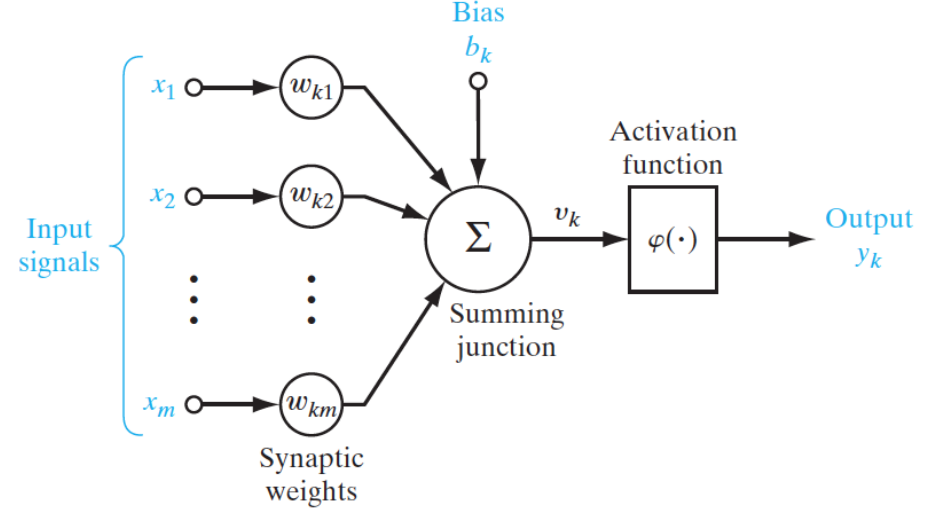
\includegraphics[width=\columnwidth]{images/neuron.png}
\end{minipage}}
%
Linear function\\
\fbox{\begin{minipage}{\linewidth}
\underline{Def.:} A function $f:\mathbf{R}^n\rightarrow\mathbf{R}$ is a linear function if:\\
$(1)\text{ }f(x+x')=f(x)+f(x'), (\forall x,x' \in \mathbf{R}^n)$\\
$(2)\text{ }f(\alpha x)=\alpha f(x), (\forall \alpha \in \mathbf{R})$
\end{minipage}}
%
\fbox{\begin{minipage}{\linewidth}
\underline{Proposition:} $f$ linear $\Leftrightarrow f(x)=w^\top x$ for some $w \in \mathbf{R}^n$.
\hrule 
$\Leftarrow$ Properties of scalar product:\\
$(1)\text{ } f(x+x')=...=f(x)+f(x')$\\
$(2)\text{ } f(\alpha x)=...=\alpha f(x)$\\
$\Leftarrow$ Write $x=\sum_{i=1}^nx_i e_i$. Linearity implies:\\
$f(\mathbf{x})=\sum_{i=1}^nx_i f(e_i)$ identify $w_i:=f(e_i)$
\end{minipage}}
%
Hyperplane\\
\fbox{\begin{minipage}{\linewidth}
\underline{Def.:} A hyperplane is an affine subspace of co-dimension 1.
\end{minipage}}
%
Level set\\
\fbox{\begin{minipage}{\linewidth}
\underline{Def.:} The level sets of a fucntion $f:\mathbf{R}^n\rightarrow \mathbf{R}$ is a one-parametric family of sets defined as \\
$L_f(c):=\{x:f(x)=c\}=f^{-1}(c)\subseteq \mathbf{R}^n$
\end{minipage}}
%
Level sets of linear functions\\
\fbox{\begin{minipage}{\linewidth}
\underline{Def.:} Let $f:\mathbf{R}^n\rightarrow \mathbf{R}$ be linear, $f(x)=w^\top x +b$, then \\
$L_f(c)=\{x:w^\top x=c-b\}=\text{hyperplane} \perp w$
\end{minipage}}
%
Linear (affine) maps\\
\fbox{\begin{minipage}{\linewidth}
$F:\mathbf{R}^n\rightarrow\mathbf{R}^m$ with \\
$F(x)=\begin{pmatrix} f_1(x)\\ f_2(x) \\...\\ f_m(x)\end{pmatrix}
= \begin{pmatrix} w_1^\top x+b_1\\ w_2^\top x+b_2 \\...\\ w_m^\top x+b_m\end{pmatrix} = \begin{pmatrix} w_1^\top \\ w_2^\top \\ ... \\ w_m^\top \end{pmatrix} x + \begin{pmatrix} b_1\\ b_2 \\...\\ b_m\end{pmatrix}$
\end{minipage}}
%
Composition of linear maps\\
\fbox{\begin{minipage}{\linewidth}
\underline{Proposition:} Let $F_1,..,F_L$ be linear maps, then $F=F_L\circ \cdots \circ F_1$ is also a linear map. Proof: $F(\mathbf{x})=(\mathbf{W}_L ...(\mathbf{W}_2(\mathbf{W}_1 \mathbf{x}))...)=(\mathbf{W}_L ... \mathbf{W}_2 \mathbf{W}_1)\mathbf{x} =\mathbf{Wx}$ \\
- every $L$-level hierarchy collapses to one level \\
- note that $rank(F)\equiv dim(im(F))\leq\min_l rank(F_l)$\\
\textbf{Conclusion: Need to move beyond linearity!}
\end{minipage}}
%
\hl{\textbf{1.5: Approximation Theory}}\\
%
Ridge function\\
\fbox{\begin{minipage}{\linewidth}
\underline{Def. (Ridge function):} $f:\mathbf{R}^n\rightarrow\mathbf{R}$ is a ridge function, if it can be written as 
$f(\mathbf{x})=\sigma(\mathbf{w}^\top \mathbf{x}+b)$ \\
- Limit set: $L_f(c)=\cup_{d\in\sigma^{-1}(c)}L_{\bar{f}}(d)$, \\if linear  part of $f$ denoted by $\bar{f}(\mathbf{x})=\mathbf{w}^\top \mathbf{x}+b$\\
- If $\sigma$ is differentiable at $z=\mathbf{w}^\top\mathbf{x}+b$ then \\
$\nabla_x f \overset{\text{chain rule}}{=} \sigma'(z)\nabla_x\bar{f}=\sigma'(z)\mathbf{w}$
\end{minipage}}
%
\fbox{\begin{minipage}{\linewidth}
\underline{Theorem} Let $f:\mathbf{R}^n\rightarrow \mathbf{R}$ differentiable at $\mathbf{x}$. Then either $\nabla f(\mathbf{x})=0$ or $\nabla f(\mathbf{x})\perp L_f(f(\mathbf{x}))$.
\end{minipage}}
%
\fbox{\begin{minipage}{\linewidth}
\underline{Def. (Dense Subsets):} A function class $\mathcal{H} \subseteq C(\mathbf{R}^d)$ is dense in $C(\mathbf{R}^d)$ iff \\
$\forall f \in C(\mathbf{R}^d) \forall \epsilon > 0 \forall K \subset \mathbf{R}^d$, compact: \\
$\exists h \in \mathcal{H} s.t. \max_{\mathbf{x}\in K}|f(\mathbf{x})-h(\mathbf{x})|=\|f-h\|_{\infty, K}<\epsilon$ \\
\textbf{Conclusion: We cann approximate any continuous $f$ to arbitrary accuracy (on K) with a suitable member of $\mathcal{H}$.} \\
- uniform approximation on compacta (i.e. use of $\infty$-norm) \\
- $\sup \rightarrow \max$ (Bolzano-Weierstrass)
\end{minipage}}
%
%\clearpage
Universal Approximation with Ridge Functions\\
\fbox{\begin{minipage}{\linewidth}
\underline{Definitions:} Let $\sigma: \mathbf{R} \rightarrow \mathbf{R}$ be a scalar function \newline
$\mathcal{G}^n_\sigma := \{g:g(\mathbf{x})=\sigma(\mathbf{w}^\top \mathbf{x}+b)$ for some $\mathbf{w}\in \mathbf{R}^n, b\in\mathbf{R}\}$ \newline
$\mathcal{G}^n := \cup_{\sigma \in C(\mathbf{R})}\mathcal{G}^n_\sigma,$ universe of continuous ridge functions
%
\textbf{\underline{Theorem:} Vostrecov and Kreines, 1961}\\
$\mathcal{H}^n := $ span$(\mathcal{G}^n)$ is dense in $C(\mathbf{R}^n)$.
\end{minipage}}
%
Dimension Lifting Lemma (Pinkus)\\
\fbox{\begin{minipage}{\linewidth}
\underline{Lemma (Pinkus 1999):} The density of $\mathcal{H}^1_\sigma$ in $C(\mathbf{R})$ with \\$\mathcal{H}^1_\sigma :=\text{span}(\mathcal{G}^1_\sigma)=\text{span}\{\sigma(\lambda t +\theta): \lambda, \theta \in \mathbf{R} \}$\\ implies the density of\\
$\mathcal{H}^n_\sigma :=\text{span}(\mathcal{G}^1_\sigma)=\text{span}\{\sigma(\mathbf{w}^\top \mathbf{x} +b):\mathbf{w}\in\mathbf{R}^n, b \in \mathbf{R} \}$\\ in $C(\mathbf{R}^n)$ for any $n\geq 1$.\\ 
\textbf{Conclusion: We can lift density property of ridge function families from $C(\mathbf{R})$ to $C(\mathbf{R}^n)$.}\\
Proof:...
\end{minipage}}
%
\fbox{\begin{minipage}{\linewidth}
- Continuous functions can be well approximated by linear combinations of ridge functions (universal function approximation). \\
- Justifies use of computational units which apply a scalar non-linearity to a linear function of the inputs.
\end{minipage}}
%
\hl{\textbf{2.1: Rectification Networks}}\\
%
\fbox{\begin{minipage}{\linewidth}
\underline{Def.:} {\color{blue} Rectified linear unit (ReLU)} \\
$(x)_+ := \max(0,x),$ \\
$\partial(x)_+ = 1 (x>0), 0 (x<0), [0;1] (x=0)$\\
\underline{Def.:} {\color{blue} Absolute value rectification (AVU)} \\
$|x|:= x(x\geq0), -x ($otw.$),$\\$\partial|x|=1(x>0),[-1;1](x=0), -1 (x<0)$
\end{minipage}}
%
Shektman (1982)\\
\fbox{\begin{minipage}{\linewidth}
Any $f\in C[0;1]$ can be uniformly approximated to arbitrary precision by a polygonal line \end{minipage}}
%
Lebesgue (1898)\\
\fbox{\begin{minipage}{\linewidth}
A polygonal line with $m$ pieces can be written \\
\fbox{$g(x) = ax + b + \sum_{i=1} ^{m-1}c_i(x-x_i)_+$}\\
\fbox{$g(x) = a'x + b' + \sum_{i=1} ^{m-1}c_i'|x-x_i|$}\\
- knots: $0=x_0 < x_1 < \cdots <x_{m-1} < x_m = 1$ \\
- $m+1$ parameters $a,b,c_i \in \mathbf{R}$ \\
- ReLU function approximation in $1$D
\end{minipage}}
\fcolorbox{black}{green}{\begin{minipage}{\linewidth}
Proof (by induction over $m$): \\
$m=1:$ Linear function over $[0;1] \Rightarrow $ fit line with $a,b$\\
$m\Rightarrow m+1:$ Given $m+1$ knots and values ($x_j,y_j$). Eliminate knot $x_m$ and choose $a,b,$ and $c_i(i<m)$ to fit this function (induction hypothesis) \\
Now modify $c_{m-1}$ and choose $c_m$ to fit a wedge to the three points ($x_{m-1},y_{m-1}$), ($x_m,y_m$), and ($x_{x+1}=1,y_{m+1}$)
\end{minipage}}
%
\fbox{\begin{minipage}{\linewidth}
- Weierstrass: $C[0;1]$ functions can be uniformly approximated by polynomials \\
- Lebesgue: proof for Weierstrass theorem by showing that $|x|$ can be uniformly approximated on $[-1;1]$ by polynomials
\end{minipage}}
%
\fbox{\begin{minipage}{\linewidth}
\underline{Theorem:} Networks with one hidden layer of ReLU or AVU are universal function approximators
\end{minipage}}
\fcolorbox{black}{green}{\begin{minipage}{\linewidth}
1. Universally approximate $C(K)$ functions ($K$, compact) by polygonal lines \\
2. Represent polygonal lines by (linear function $+$) linear combinations of $(\cdot)_+$ or $|\cdot|$ functions.\\
3. Apply dimension lifting lemma to show density of the linear span of resulting ridge function families $\mathcal{G}^n_{(\cdot)_+}$ and $\mathcal{G}^n_{|\cdot|}$
\end{minipage}}
{Linear Combinations of Rectified Units} \\
\fbox{\begin{minipage}{\linewidth}
By linearly combining $m$ rectified units, into how many ($R(m)$) cells is $\mathbf{R}^n$ maximally partioned? (Zaslavsky, 1975)\\
$R(m) \leq \sum_{i=0}^{\min\{m,n\}} \begin{pmatrix} m \\ i \end{pmatrix}$ \\
- for $m\leq n$, $R(m)=2^m$ (exponential growth)\\
- for given $n$, asymptotically, $R(m)\in\Omega(m^n)$ (bounded by $m^n$),
i.e. there is a polynomial slow-down, which is induced by the limitation of the input space dimension.
\end{minipage}}
{Deep Combinations of Rectified Units} \\
\fbox{\begin{minipage}{\linewidth}
Process $n$ inputs through $L$ ReLU layers with widths $m_1,...,m_L\in O(m)$. Into how many ($R(m,L)$) cells can $\mathbf{R}^n$ be maximally partitioned? \\
\underline{\textbf{Theorem (Montufar, 2014):}} $R(m,L)\in\Omega\left((\frac{m}{n})^{n(L-1)}m^n\right)$ \\
For any fixed $n$, exponential growth can be ensured by making layers sufficiently wide ($m>n$) and increasing the level of functional nesting (i.e. depth $L$).
\end{minipage}}
{Hinging Hyperplanes} \\
\fbox{\begin{minipage}{\linewidth}
\underline{Def.:} Hinge function: If $f:\mathbf{R}^n\rightarrow\mathbf{R}$ can be written with parameters $w_1,w_2\in\mathbf{R}^n$ and $b_1,b_2\in \mathbf{R}$ as below it is called a hinge function: 
$g(\mathbf{x})=\max(\mathbf{w}_1^\top \mathbf{x} + b_1, \mathbf{w}_2^\top \mathbf{x} + b_2)$\\
- face: $(\mathbf{w}_1-\mathbf{w}_2)^\top\mathbf{x}+(b_1-b_2)=0$\\
- representational power: $2\max(f,g)=f+g+|f-g|$\\
- k-Hinge function: $g(\mathbf{x})=\max(\mathbf{w}_1^\top \mathbf{x} + b_1,...,\mathbf{w}_k^\top \mathbf{x} + b_k)$ \\
\underline{\textbf{Theorem (Wang and Sun, 2004):}} Every continuous piecewise linear function from $\mathbf{R}^n\rightarrow\mathbf{R}$ can be written as a signed sum of $k$-Hinges with $k\leq n+1$. \\
- exact representation (not approximation as ReLU, AVU). \\
- to represent $k$-Hinge with ReLU: need depth log. in $k$.
\end{minipage}}
\begin{minipage}{\linewidth}
{Polyhedral Function (Convex functions)} \\
\fbox{\begin{minipage}{\linewidth}
= convex and continuous piecewise linear functions \\
- $f$ polyhedral $\leftrightarrow$ epi($f$) is a polyhedral set \\
- epigraph of $f$ (all points above the graph of $f$): \\ epi($f$)$:=\{(\mathbf{x},t)\in\mathbf{R}^{n+1}:f(\mathbf{x})\leq t\}$\\
- polyhedral set $S$: finite intersection of closed half-spaces\\
$S=\{\mathbf{x}\in\mathbf{R}^n:\mathbf{w}_j^\top\mathbf{x}+b_j\geq 0, j=1,...r\}$
\end{minipage}}
\end{minipage}
{Max-Representation of Polyhedral Functions} \\
\fbox{\begin{minipage}{\linewidth}
For every polyhedral $f$, there exists $\mathcal{A} \subset \mathbf{R}^{n+1}, |\mathcal{A}|=m$ s.t. \\
$f(x) = \max_{(w,b)\in \mathcal{A}}\{\mathbf{w}^\top \mathbf{x} +b \}$ \\
- each polyhedral $f$ can be repres. as max. of supp. hyperplanes \\
- linear functions in $\mathcal{A}$ describe supporting hyperplanes of epi($f$).
\end{minipage}}
{ Continuous Piecewise Linear Functions} \\
\fbox{\begin{minipage}{\linewidth}
\underline{\textbf{Theorem (Wang, 2004):}} Every continuous piecewise linear function $f$ can be written as the difference of two polyhedral functions; with finite $\mathcal{A}^+, \mathcal{A}^-$ \\
$f(x)=\max_{(w,b)\in \mathcal{A}^+}\{\mathbf{w}^\top \mathbf{x} +b \} -
\max_{(w,b)\in \mathcal{A}^-}\{\mathbf{w}^\top \mathbf{x} +b \}$
\end{minipage}}
{2 $\times$ Maxout = Allout} \\
\fbox{\begin{minipage}{\linewidth}
\underline{\textbf{Theorem (Goodfellow, 2013):}} Maxout networks with two maxout units are universal function approximators.
\end{minipage}}
%
\fcolorbox{black}{green}{\begin{minipage}{\linewidth}
1. Wang's theorem: linear network with two maxout units and a linear output unit (subtraction) can represent any continuous PWL function (exactly!).\\
2. Continuous PWL functions are dense in $C(\mathbf{R}^n)$.
\end{minipage}}
%
\hl{\textbf{2.2: Sigmoid Networks}}\\
{Sigmoid functions} \\
\fbox{\begin{minipage}{\linewidth}
$\sigma(t) = \frac{1}{1+e^{-t}}=\frac{e^t}{1+e^t}\in(0;1), \sigma^{-1}(\mu) =\ln \left(\frac{\mu}{1-\mu}\right)$ \\
$\tanh(t)=2\sigma(2t)-1\in(-1;1)$
\end{minipage}}
{Approximation Theorem} \\
\fbox{\begin{minipage}{\linewidth}
\underline{\textbf{Theorem (Lencho, Lin, Pinkus, Schocken, 1993):}} Let $\sigma\in C^\infty (\mathbf{R})$, not a polynomial, then $\mathcal{H}^1_\sigma$ is dense in $C(\mathbf{R})$; i.e. results in dense function approximation.\\
\underline{\textbf{Corollary:}} MLPs with one hidden layer and any non-polynomial, smooth activation function are universal function approximators. \\
\underline{\textbf{Lemma:}} MLPs with one hidden layer and a polynomial activation function are \textbf{not} universal function approximators. 
\end{minipage}}
\fcolorbox{black}{green}{\begin{minipage}{\linewidth}
1. For all $h\neq 0: \frac{\sigma((\lambda+h)t+\theta)-\sigma(\lambda t + \theta)}{h}\in \mathcal{H}_\sigma$\\
2. It follows that (generalizing to all k-th derivatives): \\
$\frac{d^k}{d\lambda^k}\sigma(\lambda t +\theta)|_{\lambda = 0} = t^k\sigma^{(k)}(\theta)\in cl(\mathcal{H}_\sigma)$\\
3. If we can show that there always is a $\theta_0$ such that $\sigma^{(k)}(\theta_0)\neq 0$ then we are be guaranteed that $t^k \in cl(\mathcal{H}_\sigma)$ and hence all polynomials. \\
4. By the Weierstrass theorem this implies the result\\
\underline{\textbf{Theorem (Donoghue, 1969):}} If $\sigma$ is $C^\infty$ on $(a;b)$ and it is not a polynomial thereon, then there exists a point $\theta_0\in(a;b)$ such that $\sigma^{(k)}(\theta_0)\neq 0$ for $k=0,1,2,...$.
\end{minipage}}
{Sigmoidal MLP: Approximation Guarantees} \\
\fbox{\begin{minipage}{\linewidth}
\underline{\textbf{Theorem (Barron, 1993):}} For every $F:\mathbf{R}^n\rightarrow \mathbf{R}$ with absolutely continuous Fourier transform and for every $m$ there is a function of the form $\tilde{f}_m$ such that \\
$\int_{B_r}(f(\mathbf{x} - \tilde{f}_m(\mathbf{x}))^2\mu(d\mathbf{x}) \leq O(1/ m)$\\ where $B_r=\{\mathbf{x}\in \mathbf{R}^n: \|\mathbf{x} \|\leq r \}$ and $\mu$ is any probability measure on $B_r$.\\
The residual bound does not depend on the input dimension $n$
\end{minipage}}
%
\hl{\textbf{2.3/3.1: Feedforward Networks}}\\
%
\fbox{\begin{minipage}{\linewidth}
\underline{\textbf{Def. (Feedforward networks):}} A set of computational units arranged in a DAG (directed acyclic graph).
\underline{\textbf{Def. (Hidden layer):}} A layer that is neither the input, nor the output layer.
\end{minipage}}
%
\hl{\textbf{2.4/3.2: Output Units and Objectives}}\\
%
{Loss function} \\
\fbox{\begin{minipage}{\linewidth}
\underline{\textbf{Def. (Loss function):}} A non-negative function \\
$l: \mathcal{Y}\times\mathcal{Y}\rightarrow \mathbf{R}_{\geq 0},$ $(y^*,y)\rightarrow l(\mathbf{y}^*,\mathbf{y})$, output space: $\mathcal{Y}$ \\
squared error: $\mathcal{Y}=\mathbf{R}^m, l(\mathbf{y}^*, \mathbf{y})=\|\mathbf{y}^*-\mathbf{y} \|^2_2 = \sum_{i=1}^m(y^*_i-y_i)^2$ \\
claissification error: $\mathcal{Y}=[1:m], l(\mathbf{y}^*,\mathbf{y})=1-\delta_{\mathbf{y}^*\mathbf{y}}$
\end{minipage}}
\fbox{\begin{minipage}{\linewidth}
\underline{\textbf{Def. (Expected risk (expected loss)):}}  Assume inputs and outputs are governed by a distribution $p(\mathbf{x},\mathbf{y})$ over $\mathcal{X}\times\mathcal{Y},\mathcal{X}\subset \mathbf{R}^n$. The expected risk of $F$ is given by $J^*(F)=\mathbf{E}_{x,y}[l(\mathbf{y},F(\mathbf{x})]$
\end{minipage}}
\fbox{\begin{minipage}{\linewidth}
\underline{\textbf{Def. (Training/Empirical risk):}} Assume we have a random sample of $N$ input-output pairs $\mathcal{S}_N:=\{(\mathbf{x}_i, \mathbf{y}_i)$ iid distr. $\{ p:i=1,...,N\}$.\\
The training risk of $F$ on a training sample is \\
$J(F;\mathcal{S}_N)=\frac{1}{N}\sum^N_{i=1}l(y_i,F(x_i))$\\
- training risk is the expected risk under the empirial distribution induced by the sample $\mathcal{S}_N$. 
\end{minipage}}
\fbox{\begin{minipage}{\linewidth}
\underline{\textbf{Def. (Empirical risk minimizer):}}\\ $\hat{F}(\mathcal{S}_N)=\arg\min_{F\in\mathcal{F}}J(F;\mathcal{S}_N)$ with parameter $\hat{\theta}(\mathcal{S}_N)$.
\end{minipage}}
\fbox{\begin{minipage}{\linewidth}
\underline{\textbf{Def. (Generalized linear models):}} predict the mean of the output distribution: $\mathbf{E}[y|x]=\sigma(\mathbf{w}^\top\mathbf{x})$, $\sigma$ is invertible, $\sigma^{-1}$ is the link function.
\end{minipage}}
%
Log Likelihood\\
\fbox{\begin{minipage}{\linewidth}
$J(\theta;(\mathbf{x},\mathbf{y}))=-\log p(\mathbf{y}|\mathbf{x};\theta)$
\end{minipage}}
%
Logistic Log Likelihood\\
\fbox{\begin{minipage}{\linewidth}
$J(F;(x,y))=-\log p(y|z)=-\log \sigma((2y-1)z)=\zeta((1-2y)z)$ \\
with $z:=\bar{F}(\mathbf{x})\in\mathbf{R}$, $\zeta=\log(1+\exp(\cdot))$ (soft-plus)
\end{minipage}}
%
Likelihood for logistic regression\\
\fbox{\begin{minipage}{\linewidth}
$L = \prod_{i=1}^n p(x_i)^{y_i}(1-p(x_i))^{1-y_i}$
\end{minipage}}
%
Multinomial Log Likelihood\\
\fbox{\begin{minipage}{\linewidth}
$J(F;(\mathbf{x},y))=-\log p(y|\mathbf{x};F)=-\log\left[\frac{e^{z_y}}{\sum_{i=1}^m e^{z_i}}\right]\\=-z_y+\log\sum_{i=1}^m\exp[z_i]$
with $\mathbf{z}:=\bar{F}_i(\mathbf{x})=\mathbf{w}_i^\top \mathbf{x}\in\mathbf{R}^m$
\end{minipage}}
%
\hl{ \textbf{3.3/4.1: Backpropagation}}: Exploit compositional structure\\
%
\fbox{\begin{minipage}{\linewidth}
1. perform a forward pass (for given training example ($\mathbf{x},\mathbf{y}$)) to compute activations for all units (use $\mathbf{x}$, apply $F_1$, get first hidden layer...) \\
2. compute gradient of $J$ wrt. output layer activations\\
3. iteratively propagate activation gradient information from outputs to inputs ($\rightarrow$ backpropagation)\\
4. compute local gradients of activations wrt. weights
\end{minipage}}
\fbox{\begin{minipage}{\linewidth}
Chain rule: $(f \circ g)' = (f' \circ g) \cdot g'$ \\
$\frac{d(f\circ g)}{dx}|_{x=x_0} =\frac{df}{dz}|_{z=g(x_0)} \cdot \frac{dg}{dx}|_{x=x_0} $
\end{minipage}}
Jacobi matrix \\
\fbox{\begin{minipage}{\linewidth}
$\mathbf{J}_F:=\begin{bmatrix} \nabla^\top F_1 \\  \nabla^\top F_2  \\ ...\\
 \nabla^\top F_m \end{bmatrix}
 = \begin{bmatrix} \frac{\partial F_1}{\partial x_1} & \frac{\partial F_1}{\partial x_2} & ... & \frac{\partial F_1}{\partial x_n} \\
 \frac{\partial F_2}{\partial x_1} & \frac{\partial F_2}{\partial x_2} & ... & \frac{\partial F_2}{\partial x_n}  \\
 ... & ... & ... & ...  \\
 \frac{\partial F_m}{\partial x_1} & \frac{\partial F_m}{\partial x_2} & ... & \frac{\partial F_m}{\partial x_n}  \end{bmatrix} \in \mathbf{R}^{m\times n}$ \\
for vector-valued function (map) $F:\mathbf{R}^n\rightarrow \mathbf{R}^m$
\end{minipage}}
Jacobi Matrix Chain Rule \\
\fbox{\begin{minipage}{\linewidth}
Vector-valued funtions $G:\mathbf{R}^n\rightarrow\mathbf{R}^q, F:\mathbf{R}^q\rightarrow\mathbf{R}^m$ \\
componentwise rule: \\
$\frac{\partial (F\circ G)}{\partial x_i}|_{x=x_0} = \sum_{k=1}^q \frac{\partial F_j}{\partial z_k}|_{\mathbf{z}=G(\mathbf{x}_0)}\cdot \frac{\partial G_k}{\partial x_i}|_{x=x_0}$ \\
Jacobi matrix chain rule (do not commute!) \\
$\mathbf{J}_{F\circ G}|_{x=x_0} = \mathbf{J}_F|_{z=G(x_0)} \cdot \mathbf{J}_G|_{x=x_0}$
\end{minipage}}
Function Composition \\
\fbox{\begin{minipage}{\linewidth}
$G:\mathbf{R}^n\rightarrow \mathbf{R}^m, f:\mathbf{R}^m\rightarrow\mathbf{R}, f\circ G:\mathbf{R}^n\rightarrow \mathbf{R}$ \\
$\mathbf{R}^n \ni \mathbf{x} \overset{G}{\rightarrow} \mathbf{y} \overset{f}{\rightarrow} z \in \mathbf{R}$ \\
\underline{\textbf{Lemma(Chain rule for "activations"):}} \\
\fbox{$\nabla_\mathbf{x} z = \nabla_\mathbf{y}^\top z\cdot \mathbf{J}_G,$} $\frac{\partial z}{\partial x_i} = \sum_j\frac{\partial y_j}{\partial x_i}\frac{\partial z}{\partial y_j}$ \\
$z$: output, $x$:input, for $f$ don't need Jacobian
\end{minipage}}
Activity Backpropagation \\
\fbox{\begin{minipage}{\linewidth}
$F=F^L\circ \cdots \circ F^1 :\mathbf{R}^n \rightarrow \mathbf{R}^m $ \\
$\mathbf{x}=\mathbf{x}^0 \overset{F^1}{\rightarrow} \mathbf{x}^1  \overset{F^2}{\rightarrow} \mathbf{x}^2  \rightarrow \cdots \overset{F^L}{\rightarrow}\mathbf{x}^L = \mathbf{y} \overset{\mathcal{R}}{\rightarrow} \mathcal{R}(\theta;\mathbf{y})$\\
$\nabla_\mathbf{x} J = \mathbf{J}^\top_{F^1} \cdots \mathbf{J}^\top_{F^L} \nabla_{\mathbf{y}}J$\\
Can compute all activity gradients $\nabla_{\mathbf{x}^l}$ in backward order via successive matrix multiplication with (transposed) Jacobians. \\
$\mathbf{e}^0:=\nabla_\mathbf{y}^\top \mathcal{R}$, \\
$\mathbf{e}^l:=\nabla^\top_{\mathbf{x}^l}\mathcal{R}=
\mathbf{e}^0\cdot \mathbf{J}_{F^l}\cdots \mathbf{J}_{F^{l+1}}=\mathbf{e}^{l+1}\mathbf{J}_{F^{l+1}}$
\end{minipage}}
%
\fcolorbox{black}{green}{\begin{minipage}{\linewidth}
Proof (by induction over depth $L$) \\
Base case ($L=0$): $\mathbf{x}=\mathbf{y}\Rightarrow \nabla_\mathbf{x} J = \nabla_\mathbf{y}J$\\
Induction case: $F=(F^L\circ \cdots \circ F^2)\circ F^1$\\
$\nabla_\mathbf{x} J \overset{\text{lemma}}{=}\mathbf{J}^\top_{F^1}\nabla_{\mathbf{x}^1}J\overset{IH}{=}\mathbf{J}^\top_{F^1}(\mathbf{J}^\top_{F^2}...\mathbf{J}^\top_{F^L} \nabla_\mathbf{y}J)$
\end{minipage}}
%
Jacobian for ridge function \\
\fbox{\begin{minipage}{\linewidth}
$\mathbf{x}^l=F^l(\mathbf{x}^{l-1})=\sigma(\mathbf{W}^l\mathbf{x}^{l-1}+\mathbf{b}^l)$\\
$\frac{\partial x^l_i}{\partial x^{l-1}_j}=\sigma'(\langle\mathbf{w}^l_i,\mathbf{x}^{l-1}\rangle+b^l_i)W^l_{ij}:=\bar{W}^l_{ij}$\\
thus: $\mathbf{J}_{F^l}=\mathbf{\tilde{W}}^l$
\end{minipage}}
\fbox{\begin{minipage}{\linewidth}
Multinomial Logistic Regression \\
$\mathbf{z}:=\bar{F}_i(\mathbf{x})\in\mathbf{R}^m$ \\
$J(F;(\mathbf{x},y))=-\log p(y|\mathbf{x};F)=-\log\left[\frac{e^{z_y}}{\sum_{i=1}^m e^{z_i}}\right]\\ = - z_y+\log\sum_{i=1}^m\exp[z_i]=\log\left[1+\sum_{i\neq y}\exp[z_i-z_y]\right]$\\
Multivariate logistic loss \\
$-\frac{\partial J(x,y^*)}{\partial z_y}=\frac{\partial}{\partial z_y}\left[z_{y^*}-\log\sum_i\exp[z_i] \right]\\= \delta_{yy^*} -\frac{\exp[z_y]}{\sum_i\exp[z_i]}=\delta_{yy^*}-p(y|x)$
\end{minipage}}
\fbox{\begin{minipage}{\linewidth}
Quadratic loss (neg. gradient: in what direction want to move)\\
$-\nabla_\mathbf{y}J(\mathbf{x},\mathbf{y}^*)=-\nabla_\mathbf{y}\frac{1}{2}\|\mathbf{y}^*-\mathbf{y} \|^2 = \mathbf{y}^*-\mathbf{y}$
\end{minipage}}
From Activations to Weights \\
\fbox{\begin{minipage}{\linewidth}
$\frac{\partial \mathcal{R}}{\partial W^l_{ij}}=\frac{\partial \mathcal{R}}{\partial x^l_i}\frac{\partial x^l_i}{\partial W^l_{ij}}=\frac{\partial \mathcal{R}}{\partial x^l_i}\cdot \sigma'(\langle\mathbf{w}^l_i,\mathbf{x}^{l-1}\rangle+b^l_i)\cdot x^{l-1}_j$ \\
$\frac{\partial \mathcal{R}}{\partial b^l_{i}}=\frac{\partial \mathcal{R}}{\partial x^l_i}\frac{\partial x^l_i}{\partial b^l_{i}}=\frac{\partial \mathcal{R}}{\partial x^l_i}\cdot \sigma'(\langle\mathbf{w}^l_i,\mathbf{x}^{l-1}\rangle+b^l_i)\cdot 1$ 
\end{minipage}}
\hl{\textbf{4.2: Optimization for Deep Network`s}}\\
{Gradient Descent} \\
\fbox{\begin{minipage}{\linewidth}
$\theta(t+1) \leftarrow \theta(t)-\eta \nabla_\theta J(\mathcal{S})$ \\
$\mathcal{S}$ = all training data $\Rightarrow$ steepest descent \\
$\mathcal{S}$ = mini batch of data $\Rightarrow$ SGD
\end{minipage}}
\fbox{\begin{minipage}{\linewidth}
$\theta(t+1) = \theta(t)-\eta\nabla_\theta \mathcal{R}$, cont.: $\dot{\theta}=-\nabla_\theta \mathcal{R}$ (Euler's method)
\end{minipage}}
Grad Descent Analysis (Convex objective $\mathcal{R}$)\\
\fbox{\begin{minipage}{\linewidth}
$\mathcal{R}$ has $L$-Lipschitz-continuous gradients: \\
$\mathcal{R}(\theta(t))-\mathcal{R}^* \leq \frac{2L}{t+1}\| \theta(0)-\theta^* \|^2 \in \mathbf{O}(t^{-1})$
\end{minipage}}
\fbox{\begin{minipage}{\linewidth}
$\mathcal{R}$ is $\mu$-strongly convex in $\theta$:\\
$\mathcal{R}(\theta(t))-\mathcal{R}^* \leq \left(1-\frac{\mu}{L} \right)^t \mathcal{R}(\theta(t))-\mathcal{R}^*)$\\
- exponential convergence ("linear rate")\\
- rate depends adversely on condition number $L/\mu$.
\end{minipage}}
\fbox{\begin{minipage}{\linewidth}
Lower bound (general case): $\mathbf{O}(t^{-2})$, achieved by Neterov acceleration.
\end{minipage}}
Curvature of objective function\\
\fbox{\begin{minipage}{\linewidth}
$\mathcal{R}(\theta-\eta\nabla\mathcal{R}) \overset{Taylor}{\approx} \mathcal{R}(\theta)-\eta \|\nabla\mathcal{R}\|^2+\frac{\eta^2}{2}\nabla\mathcal{R}^\top\mathbf{H}\nabla\mathcal{R}$ \\
with $\nabla\mathcal{R}^\top\mathbf{H}\nabla\mathcal{R}=\|\nabla\mathcal{R}\|^2_\mathbf{H}$, $\mathbf{H}=\nabla^2\mathcal{R}$ \\
ill-conditioning: $\frac{\eta}{2}\|\nabla\mathcal{R}\|^2_\mathbf{H} \gtrsim 
\|\nabla\mathcal{R}\|^2$
\end{minipage}}
{Least-Squares: Single Layer Linear Network}\\
\fbox{\begin{minipage}{\linewidth}
Objective: \\
$\mathcal{R}(\mathbf{A})=\mathbf{E}\|\mathbf{y}-\mathbf{A}\mathbf{x}\|^2=\Tr\mathbf{E}[(\mathbf{y}-\mathbf{A}\mathbf{x})(\mathbf{y}-\mathbf{A}\mathbf{x})^\top]$ \\
$=\Tr\mathbf{E}[\mathbf{y}\mathbf{y}^\top]+\Tr(\mathbf{A}\mathbf{E}[\mathbf{x}\mathbf{x}^\top]\mathbf{A}^\top)-2\Tr(\mathbf{A}\mathbf{E}[\mathbf{x}\mathbf{y}^\top])$\\
Gradient of objective: \\
$\nabla_\mathbf{A}\mathcal{R}=\nabla\mathbf{A}
\Tr(\mathbf{A}\mathbf{A}^\top)-2\nabla\mathbf{A}\Tr(\mathbf{A}\mathbf{\Gamma}^\top)=
2(\mathbf{A}-\mathbf{\Gamma})$
\end{minipage}}
{Least-Squares: Two Layer Linear Network ($\mathbf{A}=\mathbf{Q}\mathbf{W}$)}\\
\fbox{\begin{minipage}{\linewidth}
Objective: \\\
$\mathcal{R}(\mathbf{Q},\mathbf{W})=\text{const.}+\Tr(\mathbf{Q}\mathbf{W}\cdot (\mathbf{Q}\mathbf{W})^\top)-2\Tr(\mathbf{Q}\mathbf{W}\cdot\mathbf{\Gamma}^\top)$\\
$\frac{1}{2}\nabla_\mathbf{Q}\mathcal{R}=(\mathbf{QW})\mathbf{Q}^\top-\mathbf{\Gamma W}^\top = \mathbf{(A-\Gamma)W^\top}\in\mathbf{R}^{m\times k}$\\
$\frac{1}{2}\nabla_\mathbf{W}\mathcal{R}=\mathbf{Q\top(A-\Gamma)}\in \mathbf{R}^{k\times n}$\\
SVD of $\mathbf{\Gamma=U\Sigma V^\top}$, lin. transform: $\mathbf{\tilde{Q}=U^\top Q}$, $\mathbf{\tilde{W}=WV}$
\\
$\frac{1}{2}\nabla_\mathbf{\tilde{Q}}\mathcal{R}=\mathbf{UU^\top(\tilde{Q}\tilde{W}-\Sigma)VV^\top\tilde{W}^\top = (\tilde{Q}\tilde{W}-\Sigma)\tilde{W}^\top}$\\
$\frac{1}{2}\nabla_\mathbf{\tilde{W}}\mathcal{R}=\mathbf{\tilde{Q}^\top(\tilde{Q}\tilde{W}-\Sigma)}$\\
$\frac{1}{2}\nabla_{\mathbf{q}_r}\mathcal{R}=(\mathbf{q_r^\top w_r-\sigma_r)w_r+\sum_{s\neq r}(q^\top_r w_s)w_s}$\\
$\frac{1}{2}\nabla_{\mathbf{w}_r}\mathcal{R}=(\mathbf{q_r^\top w_r-\sigma_r)q_r+\sum_{s\neq r}(q^\top_s w_r)q_s}$\\
Equivalent energy function (guessed)
\\ $\mathcal{\tilde{R}}(\mathbf{\tilde{Q}}, \mathbf{\tilde{W}})=\mathbf{\sum_r(q_r^\top w_r -\sigma_r)^2 + \sum_{s\neq r}(q^\top_s w_r)^2}$\\
cooperation: same input-output mode weight vector align \\
competition: different mode weight vectors are decoupled
\end{minipage}}
%
\hl{ \textbf{4.3: Stochastic Gradient Descent}}\\
\fbox{\begin{minipage}{\linewidth}
Choose update direction $\mathbf{v}$ at random such that $\mathbf{E[v]}=-\nabla \mathcal{R}$\\
$\mathcal{S}_K \subseteq \mathcal{S}_N, K\leq N$\\
$\mathbf{E}\mathcal{R}(\mathcal{S}_K)=\mathcal{R}(\mathcal{S}_N) \Rightarrow \mathbf{E} \nabla\mathcal{R}(\mathcal{S}_K)=\nabla\mathcal{R}(\mathcal{S}_N)$\\
\textbf{Update step}: $\theta(t+1)=\theta(t)-\eta\nabla\mathcal{R}(t), \mathcal{R}:=\mathcal{R}(\mathcal{S}_K(t))$ \\
Convergence to optimum: convex or strongly convex objective, Lipschitz gradients, decaying learning rate $\sum_{t=1}^\infty \eta^2(t)<\infty,\sum_{t=1}^\infty \eta(t)=\infty$, e.g. $\eta(t)=Ct^{-\alpha},\frac{1}{2}<\alpha\leq 1$, iterate (Polyak) averaging \\
\textbf{Convergence rates}: \\
- strongly-convex case: $\mathcal{O}(1/t)$\\
- non-strongly convex: $\mathcal{O}(1/\sqrt{t})$
\end{minipage}}
%
%
{Heavy Ball Method} (accelerate learning)\\
\fbox{\begin{minipage}{\linewidth}
Update: $\theta(t+1)=\theta(t)-\eta\nabla\mathcal{R}+\alpha(\theta(t)-\theta(t-1)), \alpha\in[0;1)$\\
Gradients are constant $\Rightarrow$ update steps are boosted by $1/(1-\alpha)$: \\
$\eta\|\nabla J\|(1+\alpha + \alpha^2+\alpha^3+...) \rightarrow \frac{\eta \|\nabla J\|}{1-\alpha}$,
$\alpha=0.9\Rightarrow 10\times$ \\
- accelerate for high curvature, small but consistent gradient, or noisy gradients.\\
- aims to solve poor conditioning of Hessian matrix and variance in stochastic gradient.
\end{minipage}}
%
%
{AdaGrad}\\
\fbox{\begin{minipage}{\linewidth}
Consider the entire history of gradients: gradient matrix: \\
$\theta\in\mathbf{R}^d, \mathbf{G}\in\mathbf{R}^{d\times t_{max}}, g_{it}=\frac{\partial \mathcal{R}(t)}{\partial \theta_i}|_{\theta=\theta(t)}$ \\
Learning rate decays faster for weights that have seen significant updates. 
Compute (partial) row sums of $\mathbf{G}$: $\gamma^2_i(t):=\sum_{s=1}^t g_{is}^2$ \\
Adapt learning rate per parameter: \\
$\theta_i(t+1)=\theta_i(t)-\frac{\eta}{\delta + \gamma_i(t)}\nabla\mathcal{R}(t), \delta>0$ (small) \\
Non-convex variant: RMSprop (moving average, expon. weighted): 
$\gamma^2_i(t):=\sum_{s=1}^t \rho^{t-s}g^2_{is}, \rho<1$
\end{minipage}}
%
%
{BFGS/LBFGS} (advantages of Newton, without comp. burden)\\
\fbox{\begin{minipage}{\linewidth}
Newton method: $\theta(t+1)=\theta(t)-(\nabla^2\mathcal{R})^{-1}\nabla\mathcal{R}|_{\theta=\theta(t)}$ \\
BFGS: $(\nabla^2\mathcal{R})^{-1}\approx \mathbf{M}(t)$: $\theta(t+1)=\theta(t)-\eta(t)M(t)\nabla\mathcal{R}|_{\theta=\theta(t)}$ \\
where $\mathbf{M}(t+1)=\mathbf{M}(t)$ + rank one update with $\nabla\mathcal{R}$, $\eta(t)$ via line search. LBFGS: Reduce memory footprint with $\mathbf{\tilde{M}}\approx \mathbf{M}(t)$ with $k\approx 30$ rank one matrices (pairs of vectors), mini-batch
\end{minipage}}
%
{\hl{\textbf{4.4/6.1: Optimization Heuristics}}}\\
%
{Polyak averaging (Average over iterates, reduce fluctuation)}\\
\fbox{\begin{minipage}{\linewidth}
Linear (convex case): $\bar{\theta}(t) = \frac{1}{t}\sum_{s=1}^t\theta(s)$ \\
Running (non-convex): $\bar{\theta}(t) = \alpha \theta(t-1)+(1-\alpha)\theta(t), \alpha \in [0;1)$
\end{minipage}}
%
%
{Batch normalization}\\
\fbox{\begin{minipage}{\linewidth}
Hard to find suitable learning rate for all layers (strong dependencies between weights in layers exist) $\Rightarrow$ normalize the layer activations + backpropagate through normalizations\\
Fix layer $l$, fix set of example $I\subseteq [1:N]$ \\
$\mu^l_j := \frac{1}{|I|}\sum_{i\in I}(F^l_j \circ ... \circ F^1)(\mathbf{x}[i])\in\mathbf{R}^{m_l}$ \\
$\sigma^l_j:=\sqrt{\delta+\frac{1}{|I|}\sum_i (F^l_j \circ ... \circ F^1)(\mathbf{x}[i])-\mu_j)^2}, \delta >0$ \\
Normalized activities: $\mathbf{\tilde{x}}^l_j:=\frac{\mathbf{x}^l_j-\mu_j}{\sigma_j}$ \\
Regain representational power: $\mathbf{\tilde{\tilde{x}}}^l_j = \alpha_j\mathbf{\tilde{x}}^l_j + \beta_j$
\end{minipage}}
Batch normalization (simplified) \\
\fbox{\begin{minipage}{\linewidth}
1) \textbf{Input}: mini-batch of real values $X=(x_1,..,x_n)\in\mathbf{R}^n$\\
2) \textbf{Learnable parameters}: $\gamma,\beta\in\mathbf{R}$ \\
3) \textbf{Output}: $Y=(y_1,..,y_n)\in\mathbf{R}^n$, where we have \\
(a) Mini-batch mean: $\mu:=\frac{1}{n}\sum_i x_i$\\
(b) Mini-batch variance: $\sigma^2:=\frac{1}{n}\sum_i(x_i-\mu)^2$\\
(c) Normalized mini-batch (matrix form): $\hat{X}:=\frac{X-\mu}{\sqrt{\sigma^2+\epsilon}}$ \\
(d) Output: $Y=BN_{\gamma,\beta}(X):=\gamma \hat{X}+\beta$
\end{minipage}}
%
\hl{\textbf{4.4/6.2: Norm-based Regularization}}\\
%
\fbox{\begin{minipage}{\linewidth}
Regularization = Any aspect of a learning algorithm that is intended to lower the generalization error but not the training error. E.g.: Informed regularization: encode specific prior knowledge. simplicity bias: preference for simpler models (Occam's razor). Data augmentation and cross-task learning. Model averaging, e.g. ensemble methods, drop-out.
\end{minipage}}
\fbox{\begin{minipage}{\linewidth}
Standard regularization: $\mathcal{R}_\Omega(\theta;\mathcal{S})=\mathcal{R}(\theta;\mathcal{S})+\Omega(\theta)$ \\
Deep networks: $\Omega(\theta)=\frac{1}{2}\sum_{l=1}^L\mu^l\|\mathbf{W}^l\|^2_F,\mu^l\geq0$
\end{minipage}}
Weight decay \\
\fbox{\begin{minipage}{\linewidth}
Regularization based on $L_2$-norm is also called weight decay:
$ \frac{\partial\Omega}{\partial W^l_{ij}}=\mu^l w^l_{ij}$\\
weights in $l$-th layer get pulled towards zero with "gain" $\mu^l$ \\
naturally favors weights of small magnitude \\
GD update: $\theta(t+1)=(1-\mu)\cdot \theta(t)-\eta\cdot\nabla_\theta\mathcal{R}$
\end{minipage}}
Weight decay (Analysis) \\
\fbox{\begin{minipage}{\linewidth}
Taylor: $\mathcal{R}(\theta)\approx \mathcal{R}(\theta^*)+\frac{1}{2}(\theta-\theta^*)^\top\mathbf{H}(\theta-\theta^*)$, where $\mathbf{H}_\mathcal{R}$ is the Hessian of $\mathcal{R}$: 
$\mathbf{H}_\mathcal{R}=\left(\frac{\partial^2\mathcal{R}}{\partial \theta_i \partial \theta_j}\right)$, and $\mathbf{H}:=\mathbf{H}_\mathcal{R}|_{\theta=\theta^*}$\\
$\nabla_\theta \mathcal{R}_\Omega \overset{!}{=}0 $ with $\mathbf{H=Q\Lambda Q^\top}, \mathbf{\Lambda}=diag(\lambda_1,...,\lambda_d)$\\ $\Rightarrow \theta = \mathbf{Q}(\Lambda +\mu I)^{-1}\Lambda Q^\top \theta^*$ \\
- Along directions in parameter space with large eigenvalues of $\mathbf{H}$ (i.e. $\lambda_i \gg \mu$): vanishing effect \\
- Along directions in parameter space with small eigenvalues of $\mathbf{H}$ (i.e. $\lambda_i \ll \mu$): shrunk to nearly zero magnitude\\
Linear regression: $\mathcal{R}_\Omega(\theta)=\frac{1}{2}(\mathbf{X}\theta-y)^\top(\mathbf{X}\theta-y)+\frac{\mu}{2}\|\theta \|^2 \Rightarrow \theta =\mathbf{(X^\top X+\mu I)^{-1}X^\top y}$
\end{minipage}}
Regularization via Constrained Optimization \\
\fbox{\begin{minipage}{\linewidth}
$\min_{\theta:\|\theta\|\leq r}\mathcal{R}(\theta)$ \\
Optimization approach: Projected gradient descent: \\
$\theta(t+1)=\Pi_r(\theta(t)-\eta\nabla\mathcal{R}), \Pi_r(\mathbf{v}):=\min\left\{1,\frac{r}{\|\mathbf{v} \|}\right\}\mathbf{v}$ \\
Only active when weights are (too) large
\end{minipage}}
Early Stopping\\
\fbox{\begin{minipage}{\linewidth}
Stop learning after finite (small) number of iterations. E.g. use validation data to estimate risk. Stop when flat or worsening. Keep best solution.
\end{minipage}}
Early Stopping (Analysis)\\
\fbox{\begin{minipage}{\linewidth}
Taylor: $\nabla_\theta \mathcal{R}|_{\theta_0}\approx \nabla_\theta \mathcal{R}|_{\theta^*}+\mathbf{H}_{\nabla\mathcal{R}}|_{\theta^*}(\theta_0-\theta^*)=\mathbf{H}(\theta_0-\theta^*)$ \\
$(\mathbf{I}-\eta\mathbf{\Lambda})^t\overset{!}{=}\mu(\mathbf{\Lambda+\mu I})^{-1}$
which for $\eta \lambda_i \ll 1, \lambda_i \ll \mu$ can be achieved approximately via performing $t=\frac{1}{\eta \mu}$ steps. Early stopping $=$ approximate $L_2$ regularizer.
\end{minipage}}
\hl{\textbf{6.3: Dataset Augmentation}}\\
\fbox{\begin{minipage}{\linewidth}
- Generate virtual examples by applying transformations $\tau$ to each training example $(\mathbf{x,y})$ to get $(\mathbf{\tau(x),y)})$: e.g. crop, resize, rotate, reflect, add transformations through PCA. - Inject noise: to inputs, to weights (regularizing effect), to targets (soft targets, robustness wrt. label errors)
\end{minipage}}
%
Semi-supervised training (more unlabeled data)\\
\fbox{\begin{minipage}{\linewidth}
- define generative model with corresponding log-likelihood\\
- Opt. additive combination of supervised and unsupervised risk, sharing parameters
\end{minipage}}
%
Multi-Task Learning\\
\fbox{\begin{minipage}{\linewidth}
Share representations across tasks and learn jointly (i.e. minimize combined objective); 
typically: share low level representations, learn high level representations per task.
\end{minipage}}
\\
{\textbf{Ensemble Methods: Bagging}}\\
\fbox{\begin{minipage}{\linewidth}
Ensemble method that combines model trained on bootstrap samples (BS); BS $\mathcal{\tilde{S}}^k_N$: sample $N$ times from $\mathcal{S}_N$ with replacement for $k=1,..,K$; train model on $\mathcal{\tilde{S}}^k_N\rightarrow \theta^k$. \\
Prediction: average model output probabilities $p(\mathbf{y|x;\theta^k})$: \\
$p(\mathbf{y|x})=\frac{1}{K}\sum^K_{k=1}p(\mathbf{y|x};\theta^k)$
\end{minipage}}
\hl{\textbf{6.4: Dropout}}\\
\fbox{\begin{minipage}{\linewidth}
Randomly "drop" subsets of units in network; keep probability $\pi^l_i$ for unit $i$ in layer $l$. Typically: $\pi^0_i=0.8, \pi^{l\geq 1}_i=0.5$
\end{minipage}}
{\textbf{Dropout Ensembles}}\\
\fbox{\begin{minipage}{\linewidth}
Dropout realizes an ensemble $p(\mathbf{y|x})=\sum_\mathbf{Z}p(\mathbf{Z})p(\mathbf{y|x;Z})$, where $\mathbf{Z}$ denotes the binary "zeroing" mask. 
\end{minipage}}
{\textbf{Weight Rescaling}}\\
\fbox{\begin{minipage}{\linewidth}
Approximation to geometrically averaged ensemble, to avoid $10$-$20\times$ sampling blowup: 
Scale each weight $w^l_{ij}$ by probability of unit $j$ being active:
$\tilde{w}^l_{ij} \leftarrow \pi^{l-1}_j w^l_{ij}$ \\
Make sure, net input to unit $i$ is calibrated, i.e. \\
$\sum_j \tilde{w}^l_{ij}x_j \overset{\text{!}}{=}\mathbf{E_Z}\sum_j z^{l-1}_j w^l_{ij} x_j = \sum_j\pi^{l-1}_j w^l_{ij}x_j$
\end{minipage}}
\hl{\textbf{7.1: Convolutional Layers}}\\
\fbox{\begin{minipage}{\linewidth}
\textbf{Continuous Convolution}\\
$(f\ast h)(u):=\int_{-\infty}^\infty h(u-t)f(t)dt=\int_{-\infty}^\infty f(u-t)h(t)dt$ \\
\textbf{Discrete Convolution}\\
$(f\ast h)[u]:=\sum_{t=-\infty}^\infty f[t]h[u-t]$\\
$(F\ast G)[i,j]=\sum_{k=-\infty}^\infty\sum_{l=-\infty}^\infty 
F[i-k,j-l]\cdot G[k,l]$\\
Theorem: Any linear, translation-invariant transformation $T$ can be written as a convolution with a suitable $h$.\\
\textbf{Discrete Cross-Correlation} (sliding inner product)\\
$(f\star h)[u]:=\sum_{t=-\infty}^\infty f[t]h[u+t]$ \\
- Border handling: same padding, valid padding \\
- "Kernels" (across channels) form a linear map: $h:\mathbf{R}^{r^2\times d}\rightarrow\mathbf{R}^k$, where $r \times r$ is the window size (of convolution) and $d$ is the depth (RGB).\\
- Sub-sampling (strides) to reduce temporal/spatial resolution \\
- Learn multiple convolution kernels (or filters) = multiple channels 
\end{minipage}}
Toeplitz matrix \\
\fbox{\begin{minipage}{\linewidth}
A matrix $\mathbf{H}\in\mathbf{R}^{k\times n}$ is a Toeplitz matrix, if there exists $n+k-1$ numbers $c_l(l\in[-(n-1):(k-1)]\cup \mathbf{Z})$ s.t. $H_{i,j}=c_{i-j}$
$
A =
\begin{bmatrix}
  a_{0} & a_{-1} & a_{-2} & \ldots  & \ldots & a_{-(n-1)}  \\
  a_{1} & a_0    & a_{-1} & \ddots  &        & \vdots \\
  a_{2} & a_{1}  & \ddots & \ddots  & \ddots & \vdots \\ 
 \vdots & \ddots & \ddots & \ddots  & a_{-1} & a_{-2}\\
 \vdots &        & \ddots & a_{1}   & a_{0}  & a_{-1} \\
a_{n-1} & \ldots & \ldots & a_{2}   & a_{1}  & a_{0}
\end{bmatrix}\\
$
That is: $A_{i,j} = A_{i+1,j+1} = a_{i-j}$
\end{minipage}}
\fbox{\begin{minipage}{\linewidth}
$y = h \ast x =
            \begin{bmatrix}
                h_1 & 0 & \ldots & 0 & 0 \\
                h_2 & h_1 & \ldots & \vdots & \vdots \\
                h_3 & h_2 & \ldots & 0 & 0 \\
                \vdots & h_3 & \ldots & h_1 & 0 \\
                h_{m-1} & \vdots & \ldots & h_2 & h_1 \\
                h_m & h_{m-1} & \vdots & \vdots & h_2 \\
                0 & h_m & \ldots & h_{m-2} & \vdots \\
                0 & 0 & \ldots & h_{m-1} & h_{m-2} \\
                \vdots & \vdots & \vdots & h_m & h_{m-1} \\
                0 & 0 & 0 & \ldots & h_m
            \end{bmatrix}
            \begin{bmatrix}
                x_1 \\
                x_2 \\
                x_3 \\
                \vdots \\
                x_n
            \end{bmatrix}
$\\
$\mathbf{H}^h_n\in\mathbf{R}^{(n+m-1)\times n}$.
\end{minipage}}
Backpropagation\\
\fbox{\begin{minipage}{\linewidth}
Exploit structural sparseness in computing $\frac{\partial x^l_i}{\partial x^{l-1}_j}$ \\
Receptive field of $x^l_i: \mathcal{I}^l_i:=\{j:W^l_{ij}\neq 0 \}$, where $\mathbf{W}^l$ is the Toeplitz matrix of the convolution; also $\frac{\partial x^l_i}{\partial x^{l-1}_j}=0$ for $j\notin \mathcal{I}^l_i$  \\
Weight sharing in computing $\frac{\mathcal{R}}{\partial h^l_j}$ where $h^l_j$ is a kernel weight:\\
$\frac{\mathcal{R}}{\partial h^l_j}=\sum_i \frac{\mathcal{R}}{\partial x^l_i} \frac{\partial x^l_i}{\partial h^l_i}$, weight is re-used for every unit within target layer $\Rightarrow$ additive combination
\end{minipage}}
%
CNNs (dimension)\\
\fbox{\begin{minipage}{\linewidth}
CNN
input: $H_1 \times W_1 \times C_1$, output of conv. layer with $N$ filters, kernel size $K$, stride $S$ and zero padding $P$:\\
$H2=(H_1 - K +2P)/S+1$, $W_2=(W_1-K+2P)/S+1$, $C_2=N$ \hrule
$H2=(H_1 - K)/S+1$, $W_2=(W_1-K)/S+1$, $C_2=C_1$
\end{minipage}}
%
BProp: Single input channel, single output channel\\
\fbox{\begin{minipage}{\linewidth}
input $x\in\mathbf{R}^{d\times d}$, weights $w\in\mathbf{R}^{k\times k}$ \\
output (before nonlinearity) $y=x * w$ \\
$\frac{\partial \mathcal{L}}{\partial w_{uv}}=\sum_{i}\sum_j \frac{\partial \mathcal{L}}{\partial y_{ij}}\frac{\partial y_{ij}}{\partial w_{uv}}$\\
$=\sum_{i}\sum_j \partial \delta_{ij}\frac{\partial}{\partial w_{uv}}\sum_a\sum_b x_{i-a,j-b}w_{ab}$\\
$=\sum_{i}\sum_j \partial \delta_{ij} x_{i-u,j-v} $\\$= \sum_i\sum_j \text{rot}_{180}(x_{u-i,v-j})\delta_{ij}=(\text{rot}_{180}(x)*\delta)_{u,v}$ \\
$\frac{\partial \mathcal{L}}{\partial x_{uv}}=\sum_i \sum_j \frac{\partial \mathcal{L}}{\partial y_{ij}}\frac{\partial y_{ij}}{\partial x_{ij}}=\ldots=(\text{rot}_{180}(w)*\delta)_{u,v}$
\end{minipage}}
FFT (compute convolutions faster, $\mathbf{O}(n\log n)$)\\
\fbox{\begin{minipage}{\linewidth}
$(f * h)=\mathcal{F}^{-1}((\mathcal{F}f))\cdot(\mathcal{F}h))$;
pays off if many channels; small kernels ($m < \log n$): favor time/space domain
\end{minipage}}
Convolutional Layers: Stages\\
\fbox{\begin{minipage}{\linewidth}
Input to layer $\rightarrow$ Convolution stage: affine transform $\rightarrow$ Detector stage: nonlinearity (e.g. rectified linear) $\rightarrow$ pooling stage (locally combine activities) $\rightarrow$ next layer
\end{minipage}}
Max Pooling\\
\fbox{\begin{minipage}{\linewidth}
Maximum over a small "patch" of units: \\
$1D: x^{max}_i = \max\{x_{i+k}:0\leq k < r\}$\\
$2D: x^{max}_{ij} = \max\{x_{i+k,j+l}:0\leq k,l < r\}$ \\
$\mathcal{T}$-invariance through maximization $f_\mathcal{T}(\mathbf{x}):=\max_{\tau\in\mathcal{T}}f(\tau \mathbf{x})$ \\
$f_\mathcal{T}$ is invariant under $\tau\in\mathcal{T}$: $f_\mathcal{T}(\tau\mathbf{x})=\max_{\rho\in\mathcal{T}}f(\rho(\tau\mathbf{x}))=
\max_{\rho\in\mathcal{T}}f((\rho\circ\tau)\mathbf{x})=\max_{\sigma\in\mathcal{T}}f(\sigma \mathbf{x})$,
as $\forall \sigma, \sigma=\rho\circ\tau$ with $\rho=\sigma\circ\tau^{-1}$
\end{minipage}}
\hl{\textbf{8.1: Conv. Networks for Natural Language}}\\
Point-wise mutual information (pmi)\\
\fbox{\begin{minipage}{\linewidth}
$\text{pmi}(v,w)=\log\frac{p(v,w)}{p(v)p(w)}=\log\frac{p(v|w}{p(v)}=\mathbf{x}\top\mathbf{x}_w+\text{const}.$
\end{minipage}}
Skip-gram objective\\
\fbox{\begin{minipage}{\linewidth}
$\mathcal{L}(\theta;\mathbf{w})=\sum_{(i,j)\in\mathcal{C_R}}\log
\left[\frac{p_\theta(w_i|w_j)}{p(w_i)} \right]$ with\\
co-occurence index set $\mathcal{C}_R:=\{(i,j)\in[1:T]^2:1\leq |i-j|\leq R \}$
\end{minipage}}
Skip-gram model (soft-max)\\
\fbox{\begin{minipage}{\linewidth}
$\log p_\theta(v|w)=\mathbf{x}^\top_v\mathbf{z}_w-\log\sum_{u\in\mathcal{V}}
\exp[\mathbf{x}^\top_u\mathbf{z}_w]$
\end{minipage}}
Skip-gram model (negative sampling, logistic regression)\\
\fbox{\begin{minipage}{\linewidth}
$\mathcal{L}(\theta;\mathbf{w})=\sum_{(i,j)\in\mathcal{C_R}}\left[\log\sigma
(\mathbf{x}^\top_{w_i}\mathbf{z}_{w_j})+k\mathbf{E}_{v\sim p_n}[\log\sigma(-\mathbf{x}^\top_{w_i}\mathbf{z}_{w_j})] \right]$
\end{minipage}}
\hl{ \textbf{8.2: Recurrent Networks}}\\
\fbox{\begin{minipage}{\linewidth}
- Markov property \\
- Time-invariance, share weights \\
$\bar{F}(h,x;\theta):=Wh+Ux+b$ \\
$y=H(h;\theta), H(h;\theta):=\sigma(Vh+c)$
\end{minipage}}
%
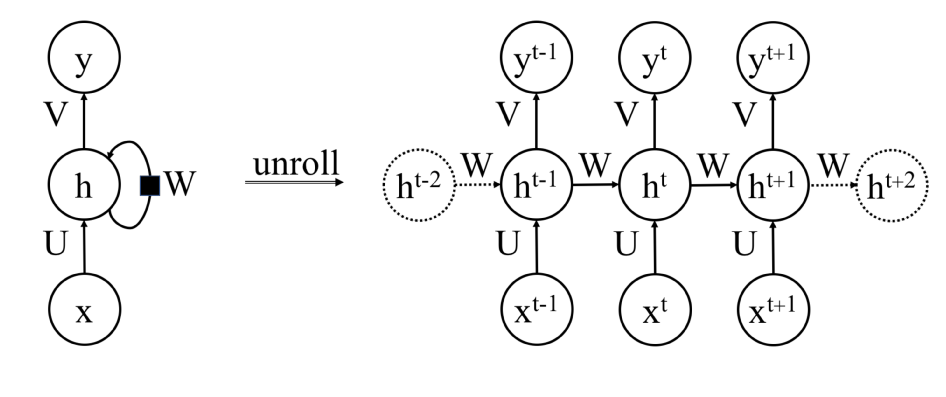
\includegraphics[width=0.8\columnwidth]{images/rnn.png} \\
\fbox{\begin{minipage}{\linewidth}
Backpropagation \\
$\frac{\partial \mathcal{R}}{\partial w_{ij}}=\sum_{t=1}^T\frac{\partial\mathcal{R}}{\partial h^t_i}\frac{\partial h^t_i}{\partial w_{ij}} = \sum_{t=1}^T\frac{\partial \mathcal{R}}{\partial h^t_i}\cdot \dot{\sigma}^t_i \cdot h^{t-1}_j$ \\
$\frac{\partial \mathcal{R}}{\partial u_{ik}}=\sum_{t=1}^T\frac{\partial\mathcal{R}}{\partial h^t_i}\frac{\partial h^t_i}{\partial u_{ik}} = \sum_{t=1}^T\frac{\partial \mathcal{R}}{\partial h^t_i}\cdot \dot{\sigma}^t_i \cdot x^t_k$ \\
with $\dot{\sigma}^t_i :=\sigma'(\bar{F}_i(h^{t-1},x^t))$\\
MLP: $\nabla_\mathbf{x}\mathcal{R}=\mathbf{J}_{F^1} ....\mathbf{J}_{F^L}\nabla_\mathbf{y}\mathcal{R}$ \\
RNN $(F^t=F)$: $\nabla_{\mathbf{x}^t}\mathcal{R} = \left[\prod_{s=t+1}^T \mathbf{W}^\top\mathbf{S}(\mathbf{h}^s) \right]\cdot \mathbf{J}_H\nabla_\mathbf{y}\mathcal{R}$ \\
where $\mathbf{S}(\mathbf{h}^s)=diag(\dot{\sigma}^s_1,...,\dot{\sigma}^s_n)$
\end{minipage}}
Loss depends on all outputs\\
\fbox{\begin{minipage}{\linewidth}
loss $L=\sum_{t=1}^T L_t$, input $\mathbf{x}^t$, state $\mathbf{h}^t$: \\
$\mathbf{h}^t=F(\mathbf{h}^{t-1},\mathbf{x}^t,\theta)=\alpha(\mathbf{W}\mathbf{h}^{t-1}+\mathbf{U}\mathbf{x}^t
+\mathbf{b})$ \\
$\frac{\partial L}{\partial \theta}=\sum_{t=1}^T\frac{\partial}{\partial \theta} L_t $\\
Sum over all the paths in the (unfolded) network leading from the parameters to the loss:
$\frac{\partial L_t}{\partial \theta}=\sum_{k=1}^t \frac{\partial L_t}{\partial h_t}\frac{\partial h_t}{\partial h_k} \frac{\partial h_k}{\partial \theta}$\\
Expansion along a single path: \\
$\frac{\partial h_t}{\partial h_k}=\prod_{i=k}^t\frac{\partial h_i}{\partial h_{i-1}}=\prod_{i=k}^tW^\top \text{diag}(\alpha'(\cdot))$
\end{minipage}}
Loss depends only on last output \\
\fbox{\begin{minipage}{\linewidth}
$\bar{h}_t=F(x_t,x_{t-1};\theta)$ \\
$h_t=\sigma(t)$\\
$y_t=G(h_t;\kappa)$\\
$L_T:=L(y_T)+\frac{\lambda}{2}\|\theta\|_2^2$\\
$\frac{\partial L_T}{\partial \theta} = \frac{\partial L(y_T)}{\partial \theta}+\lambda$ \\
$=\frac{\partial L(y_T)}{\partial y_T}\frac{\partial G(h_T;\kappa)}{\partial h_T}\sum_{k=t}^T\frac{\partial h_T}{\partial h_t}\frac{\partial h_t}{\partial \theta}$\\
$=\frac{\partial L(y_T)}{\partial y_T}\frac{\partial G(h_T;\kappa)}{\partial h_T}\sum_{k=t}^T\prod\frac{\partial h_T}{\partial h_t}\frac{\partial h_t}{\partial\theta}$
\end{minipage}}
Bi-Directional Recurrent Networks\\
\fbox{\begin{minipage}{\linewidth}
$g^t=G(x^t,g^{t+1};\theta)$ \\
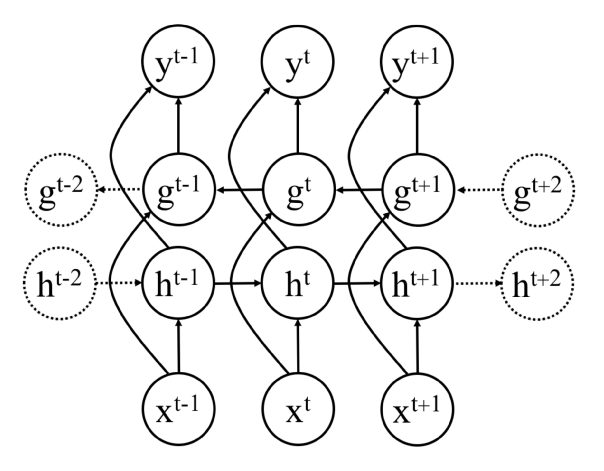
\includegraphics[width=0.5\columnwidth]{images/bi_rnn.png}
\end{minipage}}
%
Deep Recurrent Networks\\
\fbox{\begin{minipage}{\linewidth}
$h^{t,1}=F^1(h^{t-1,1},x^t;\theta)$\\
$h^{t,l}=F^l(h^{t-1,l},h^{t,l-1};\theta), l=2,...,L$ \\
$y^t=H(h^{t,L};\theta)$\\
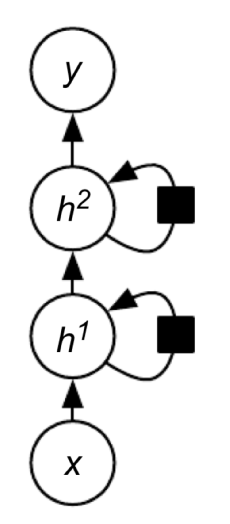
\includegraphics[width=0.2\columnwidth]{images/deep_rnn.png}
\end{minipage}}
\hl{\textbf{9.1: Memory Units}}\\
LSTM \\
\fbox{\begin{minipage}{\linewidth}
input processing (1), input g. (2), forget g. (3), output g. (4)\\
$F^\kappa = \sigma \circ \bar{F}^\kappa $, $\bar{F}^\kappa = W^\kappa h^{t-1} + U^\kappa x^t+ b^\kappa, \kappa\in\{1,2,3,4\}$ \\
Next state: $h^t=F^3(...)\circ h^{t-1}+F^2(...)\circ F^1(...)$ \\
Output: $y^t=F^4(...)\circ \tanh(h^t)$
\end{minipage}}
\fbox{\begin{minipage}{\linewidth}
= building unit for RNN. A common LSTM unit is composed of a cell, an input gate, an output gate, and a forget gate. \\
$f_t = \sigma_g(W_{f} x_t + U_{f} h_{t-1} + b_f) \in R^h \text{ (forget gate)}\\
i_t = \sigma_g(W_{i} x_t + U_{i} h_{t-1} + b_i) \in R^h \text{ (input gate)}\\
o_t = \sigma_g(W_{o} x_t + U_{o} h_{t-1} + b_o) \in R^h \text{ (output gate)}\\
c_t = f_t \circ c_{t-1} + i_t \circ \sigma_c(W_{c} x_t + U_{c} h_{t-1} + b_c) \text{ (cell state)}\\
h_t = o_t \circ \sigma_h(c_t) \text{ (output vector)}$\\
$W \in R^{h \times d}$, $U \in R^{h \times h} $ and $ \in R^{h}$: weight matrices and bias vector parameters which need to be learned during training \\
$x_t \in R^{d}:$ input vector to the LSTM unit\\
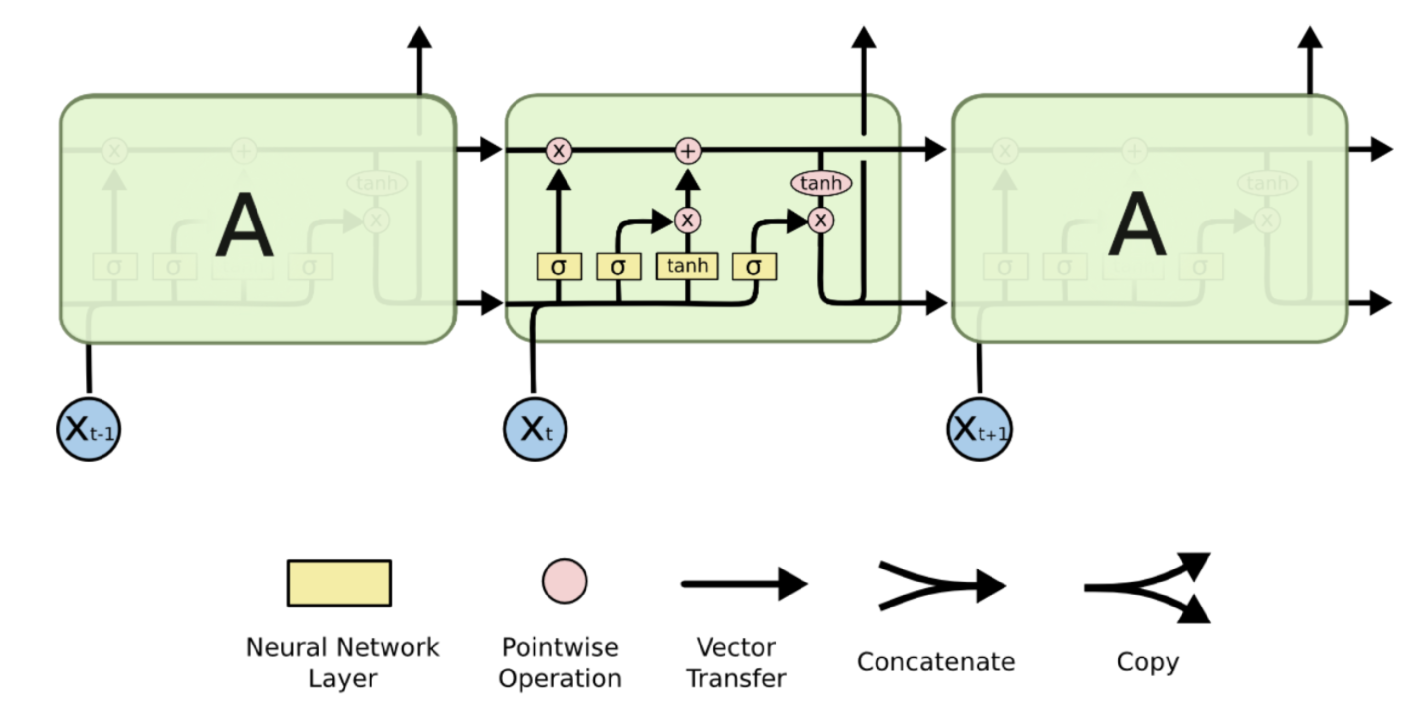
\includegraphics[width=\columnwidth]{images/LSTM.png}
\end{minipage}}
\fbox{\begin{minipage}{\linewidth}
Peephole connections allow the gates to access the constant error carousel (CEC), whose activation is the cell state. $h_{t-1}$  is not used, $c_{t-1}$ is used instead in most places.\\
$f_t = \sigma_g(W_{f} x_t + U_{f} c_{t-1} + b_f) \\
i_t = \sigma_g(W_{i} x_t + U_{i} c_{t-1} + b_i) \\
o_t = \sigma_g(W_{o} x_t + U_{o} c_{t-1} + b_o) \\
c_t = f_t \circ c_{t-1} + i_t \circ \sigma_c(W_{c} x_t + b_c) \\
h_t = o_t \circ \sigma_h(c_t)$
\begin{center}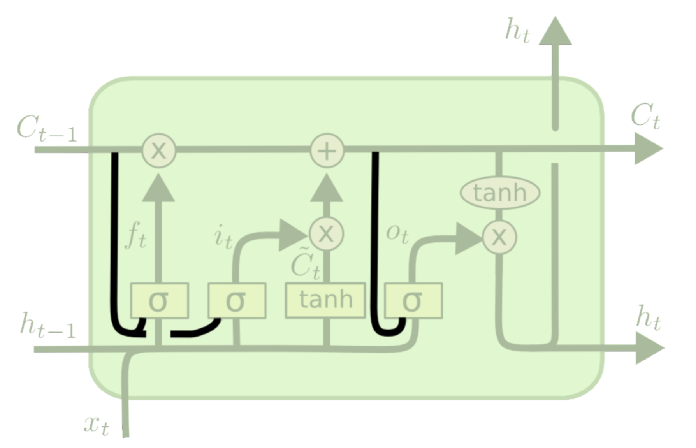
\includegraphics[width=0.5\columnwidth]{images/LSTM_peephole.png}\end{center}
\end{minipage}}\\
Gated Memory Units \\
\fbox{\begin{minipage}{\linewidth}
Memory state = output (lack output gate) \\
$z_t = \sigma_g(W_{z} x_t + U_{z} h_{t-1} + b_z) \\
r_t = \sigma_g(W_{r} x_t + U_{r} h_{t-1} + b_r) \\
h_t =  z_t \circ h_{t-1} + (1-z_t) \circ \sigma_h(W_{h} x_t + U_{h} (r_t \circ h_{t-1}) + b_h)$
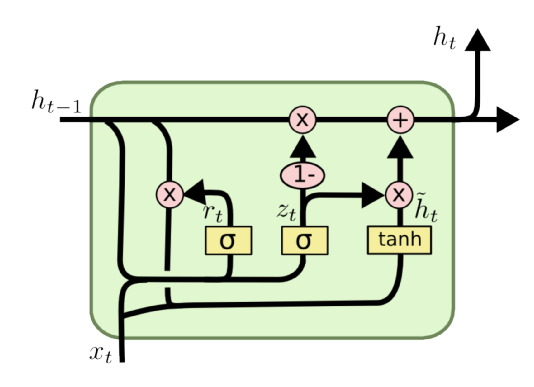
\includegraphics[width=0.4\columnwidth]{images/GRU.png}
\end{minipage}}\\
\hl{\textbf{9.2: Differentiable Memory/Neural Turing Machine}}\\
\fbox{\begin{minipage}{\linewidth}
- Able to learn to read from and write arbitrary content to memory cells. \\
- To read, they take a weighted average of many cells. \\
$r\leftarrow \sum_i \alpha_i M_i,
\alpha\geq 0, \sum_i\alpha_i = 1$\\
- To write, they modify multiple cells by different amounts. \\
$M_i \leftarrow (1-\beta_i) M_i+\beta_i w, \beta_i\in[0;1]$\\
- Weights with nonzero derivatives (softmax) enables the functions controlling access to the memory to be optimized using GD.
\end{minipage}}
\hl{\textbf{9.3: Attention}}\\
\fbox{\begin{minipage}{\linewidth}
Selectively attend to inputs or feature representations computed from inputs; select what is relevant from the past in hindsight
\end{minipage}}
\hl{\textbf{9.4: Recursive Networks}}\\
\fbox{\begin{minipage}{\linewidth}
For a sequence of length $\tau$, the depth can be reduced from $\tau$ to $O(\log \tau)$.
\end{minipage}}
\hl{\textbf{10.1: Autoencoders}}\\
\fbox{\begin{minipage}{\linewidth}
Linear auto-encoding (hidden layer $\mathbf{z}\in\mathbf{R}^m$, input dimension $n$, data points $i=1,...,k$)\\
$\mathbf{x}\in\mathbf{R}^n\overset{\mathbf{C}}{\rightarrow}\mathbf{z}\in\mathbf{R}^m (m\leq n)\overset{\mathbf{D}}{\rightarrow}\mathbf{\hat{x}}\in\mathbf{R}^n
\overset{\mathcal{R}}{\rightarrow}\frac{1}{2}\|\mathbf{x}-\mathbf{\hat{x}}\|^2$\\
Optimal choice of $\mathbf{C}\in\mathbf{R}^{n\times m}$ and $\mathbf{D}\in\mathbf{R}^{m\times n}$ s.t. \\
$\frac{1}{2k}\sum_{k=1}^k\|\mathbf{x}_i-\mathbf{D}\mathbf{C}\mathbf{x}_i\|^2\leftarrow \min$ 
\end{minipage}}
Eckart-Young Theorem (for $m\leq \min(n,k)$)\\
\fbox{\begin{minipage}{\linewidth}
$\arg\min_{\mathbf{\hat{X}}:rank(\mathbf{\hat{X}})=m}\|\mathbf{X}-\mathbf{\hat{X}}\|^2_F=\mathbf{U}_m \cdot diag(\sigma_1,...,\sigma_m)\cdot \mathbf{V}^\top_m$ \\
No linear auto-encoder with $m$ hidden units can improve on SVD as $\text{rank}(CD)\leq m$ \\
Given data $\mathbf{X}=\mathbf{U} diag(\sigma_1,..,\sigma_n)\mathbf{V}^\top$. The choice $\mathbf{C}=\mathbf{U}^\top_m$ and $\mathbf{D}=\mathbf{U}_m$ minimizes the squared reconstruction error of a two layer linear eauto-encoder with $m$ hidden units. \\
$\tilde{D} \tilde{C} = (U_m A^{-1}) \cdot (A U_m^\top) = U_m U_m^\top$ \\
Solutions restricted to $\mathbf{D}=\mathbf{C}^\top$ (weight-sharing)\\
$\Rightarrow A^{-1}=A^\top$ (orthogonal) \\
$\Rightarrow$ mapping $x\rightarrow z$ only determined up to rotations.
\end{minipage}}
Non-linear auto-encoder\\
\fbox{\begin{minipage}{\linewidth}
$\min \mathbf{E}_\mathbf{x}[l(\mathbf{x},(H\circ G)(\mathbf{x})]$, e.g. $l(\mathbf{x},\mathbf{\hat{x}})=\frac{1}{2} \|\mathbf{x}-\mathbf{\hat{x}} \|^2$\\
Encoder: $G=F_l\circ \cdots \circ F_1:\mathbf{R}^n\rightarrow \mathbf{R}^m, \mathbf{x}\rightarrow \mathbf{z}:=\mathbf{x}^l$ \\
Decoder: $H=F_L\circ \cdots \circ F_{l+1}:\mathbf{R}^m\rightarrow \mathbf{R}^n, \mathbf{z}\rightarrow \mathbf{y}:=\mathbf{\hat{x}}$
\end{minipage}}
Denoising non-linear auto-encoder\\
\fbox{\begin{minipage}{\linewidth}
$\min \mathbf{E}_\mathbf{x}\mathbf{E}_\mathbf{\eta}[l(\mathbf{x},(H\circ G)(\mathbf{x_\eta})]$
with $\mathbf{x}_\eta = \mathbf{x}+\mathbf{\eta}$, $\eta\sim\mathcal{N}(\mathbf{0},\sigma^2\mathbf{I})$
\end{minipage}}
Denoising non-linear auto-encoder\\
\fbox{\begin{minipage}{\linewidth}
code sparseness (sparse activity vector): $\Omega(\mathbf{z})=\lambda \|\mathbf{z}\|_1$ \\
contractive AE (stable wrt. changes in input): $\Omega(\mathbf{z})=\lambda \|\frac{\partial\mathbf{z}}{\partial \mathbf{x}}\|^2_F$
\end{minipage}}
\hl{\textbf{10.2: Factor Analysis}}\\
\fbox{\begin{minipage}{\linewidth}
$x=\mu+Wz+\eta$, $z\sim\mathcal{N}(0,I), \eta\sim\mathcal{N}(0,\Sigma)$ then \\
$x\sim\mathcal{N}(\mu,WW^\top+\Sigma)$, posterior $p(z|x)=\mathcal{N}(\mu_{z|x}, \Sigma_{z|x})$ \\
$\mu_{z|x}=(W^\top(WW^\top+\Sigma)^{-1}(x-\mu)$\\ $\Sigma_{z|x}=I-W\top(WW^\top+\Sigma)^{-1}W$ \\
Pseudo-inverse: $W^\dagger:=W^\top(WW^\top+\sigma^2 I)^{-1}$ for $\sigma^2\rightarrow 0$ \\
$W^\dagger=W^\top$ if $W$ orthogonal columns
\end{minipage}}
\hl{\textbf{Moment generating functions}}\\
\fbox{\begin{minipage}{\linewidth}
MGF of random vector $\mathbf{x}$: $M_\mathbf{x}:\mathbf{R}^n\rightarrow\mathbf{R}, M_\mathbf{x}:=\mathbf{E}_x\exp[\mathbf{t}^T\mathbf{x}]$\\
Uniqueness thereom: If $M_x,M_y$ exist for RVs $\mathbf{x}, \mathbf{y}$ and $M_x=M_y$ then (essentially) $p(\mathbf{x})=p(\mathbf{y})$. \\
$\mathbf{E}[x^{k_1}_1 \cdot x^{k_n}_n] = \frac{\partial^k}{\partial t^{k_1}_1 ... \partial t_n^{k_n}}M_\mathbf{x}|_{t=0}$ \\
$\mathbf{Ex}=\mu$, 
$\Sigma=\mathbf{E}(\mathbf{x}-\mathbf{\mu})(\mathbf{x}-\mathbf{\mu})^\top$ \\
PDF: $p(\mathbf{x};\mathbf{\mu},\mathbf{\Sigma}) = \frac{\exp[-\frac{1}{2}(\mathbf{x}-\mathbf{\mu})^\top\mathbf{\Sigma}^{-1}(\mathbf{x}-\mathbf{\mu})]}{\sqrt{(2\pi)^n\cdot \det{\mathbf{\Sigma}}}}$, \\
MGF: $M_x(\mathbf{t})=\exp[\mathbf{t}^\top\mu + \frac{1}{2}\mathbf{t}^\top\mathbf{\Sigma}\mathbf{t}]$
\end{minipage}}
\hl{\textbf{10.3: Deep Latent Gaussian Models (DLGMs)}}\\
\fbox{\begin{minipage}{\linewidth}
Noise variables $\mathbf{z}^l \overset{iid}{\sim}\mathcal{N}(\mathbf{0},\mathbf{I}), l=1,...L$ \\
Hidden activities (top-down: $\mathbf{h}^L\rightarrow \mathbf{h}^1$)\\
$\mathbf{h}^L=\mathbf{W}^L\mathbf{z}^L$, $\mathbf{h}^l=F^l(\mathbf{h}^{l+1})+\mathbf{W}^l\mathbf{z}^l$ \\
Hidden layer (conditional) distribution \\
$h|h^+\sim\mathcal{N}(F(\mathbf{h}^+),\mathbf{WW^\top})$\\
Recognition model: 
$\mathbf{x}\overset{\vartheta}{\rightarrow}(\mathbf{\mu}^l,\mathbf{\Sigma}^l)^L_{l=1} \rightarrow q\sim\mathcal{N}(...)$
\end{minipage}}
Jensen's inequality\\
\fbox{\begin{minipage}{\linewidth}
If $g$ is a real-valued function that is $\mu$-integrable, and if $\varphi$ is a convex function, then: 
$\varphi(\int_\Omega g d \mu) \leq \int_\Omega \varphi \circ g d\mu$
\end{minipage}}
ELBO: Evidence lower BOund\\
\fbox{\begin{minipage}{\linewidth}
$-\log p_\theta(\mathbf{x}) = - \log \int p_\theta(\mathbf{x}|\mathbf{z})p(\mathbf{z})d\mathbf{z}$\\
$=- \log \int q(\mathbf{x})\left[p_\theta(\mathbf{x}|\mathbf{z})\frac{p(\mathbf{z})}{q(\mathbf{z})}\right]d\mathbf{z}$ \\
$\leq -\int q(\mathbf{z})\log p_\theta (\mathbf{x}|\mathbf{z})d\mathbf{z} +\int q(\mathbf{z})\log \frac{q(\mathbf{z})}{p(\mathbf{z})}d\mathbf{z} =:\mathcal{F}(\theta,q;x)$ \\
$D_{KL}(q||p)=\int q(\mathbf{z})\log \frac{q(\mathbf{z})}{p(\mathbf{z})}d\mathbf{z}$
\end{minipage}}
\fbox{\begin{minipage}{\linewidth}
$\log p_\theta(\mathbf{x}) \geq \mathbf{E}_q[\log p_\theta(\mathbf{x},\mathbf{z})]+KL(q(\mathbf{z})||p_\theta(\mathbf{z}))\overset{\max\mathbf{E}}{\leftarrow}\theta,q$ \\
$q$ variational distr. approx. true intractable posterior $p(\mathbf{z}|\mathbf{x})$ \\
optimal $q(\mathbf{z};\mathbf{x})=p_\theta(\mathbf{z}|\mathbf{x}) (\text{posterior})$
\end{minipage}}
Stochastic Backpropagation\\
\fbox{\begin{minipage}{\linewidth}
$\mathbf{z}\sim\mathcal{N}(\mathbf{\mu},\mathbf{\Sigma}),$ $f$: smooth and integrable, then \\
$\nabla_\mathbf{\mu}\mathbf{E}f(\mathbf{z})]=\mathbf{E}[\nabla_\mathbf{z}f(\mathbf{z})]$,
$\nabla_\mathbf{\Sigma}\mathbf{E}[f(\mathbf{z})]=\frac{1}{2}\mathbf{E}[\nabla^2_\mathbf{z}f(\mathbf{z})]$
\end{minipage}}
\hl{\textbf{11.1: Density Estimation}}\\
\fbox{\begin{minipage}{\linewidth}
Prescribed model: Use observer likelihoods and assume observation noise \\
Implicit models: Likelihood-free models
\end{minipage}}
%
Partition Function\\
\fbox{\begin{minipage}{\linewidth}
$p(x;\theta)=\frac{1}{Z(\theta)}\tilde{p}(x;\theta)=\frac{1}{\sum_x \tilde{p}(x)}\tilde{p}(x;\theta)$\\
$\nabla_\theta \log p(x;\theta)=\nabla_\theta \log \tilde{p}(x;\theta)-\nabla_\theta \log Z(\theta)$\\
$\nabla_\theta \log Z(\theta)=\mathbf{E}_{x\sim p(x)}\nabla_\theta \log \tilde{p}(x)$
\end{minipage}}
%
Score Matching (Alternative to MLE)\\
\fbox{\begin{minipage}{\linewidth}
avoids computing quantities related to the partition function \\
score = 
$\nabla_x\log p(x)$\\
Minimize the expected squared difference between the derivatives of the model's log density wrt the input and the derivatives of the data's log density wrt the input:\\
$\psi_\theta:=\nabla \log \bar{p}_\theta, \psi=\nabla \log p$, minimize $J(\theta)=\mathbf{E}\|\psi_\theta-\psi\|^2$ \\
$J(\theta)\overset{\pm c}{=}\mathbf{E}\left[\sum_i \partial_i \psi_{\theta,i} -\frac{1}{2}\psi^2_{\theta,i} \right]$\\
+ partition function $Z$ is not a function of $x \Rightarrow \nabla_\mathbf{x}Z=0$ \\
- not applicable to models of discrete data \\
- need to evaluate $\log\tilde{p}(x)$ and its derivatives\\
- not compatible if only lower bound available 
\end{minipage}}
Noise Constrastive Estimation (NCE)\\
\fbox{\begin{minipage}{\linewidth}
The probability distribution estimated by the model is represented explicitly as 
$\log p_\text{model}(x)=\log \tilde{p}_\text{model}(x;\theta) +c$ where $c$ approximates $-\log Z(\theta)$.\\
reduces density estimation to binary classification \\
$\tilde{p}(\mathbf{x},y=1)=\frac{1}{2}p_\text{model}(x), \tilde{p}(\mathbf{x},y=0)=\frac{1}{2}p_\text{noise}(\mathbf{x})$ \\
$y$ is a switch variable that determines whether we will generate $x$ from the model or from the noise distribution\\
prob. classifier: $q_\theta = \frac{\alpha \bar{p}_\theta}{\alpha \bar{p}_\theta + p_n}$, $\alpha>0$, $p_n$: constrastive distr.\\
Bayes optimal if $\alpha \bar{p}_\theta = p$ \\
- does not work with lower bound \\
+ estimator for $\theta$ consistent as long as $p_n$ is dominating $p$ \\
- Generally not statistically efficient; much worse thatn Cramer-Rao bound if $p_n$ very different from $p$.
\end{minipage}}
\hl{\textbf{11.2: Generative Adversarial Models}}\\
\fbox{\begin{minipage}{\linewidth}
Generator: gen. samples that are indistinguishable from real data. Train by minimizing logistic likelihood: \\
$l^*(\theta):=\mathbf{E}_{\tilde{p}_\theta}[y\ln q_\theta(\mathbf{x})+(1-y)\ln(1-q_\theta(x))]$ \hrule
Classification model: $q_\phi : \mathbf{x}\rightarrow [0;1], \phi \in \mathbf{\Phi}$ \\
$l^*(\theta) \geq \sup_{\phi\in\Phi}l(\theta,\phi)$ \\
$l(\theta,\phi):=\mathbf{E}_{\tilde{p}_\theta}[y \ln q_\phi(\mathbf{x})+(1-y)\ln(1-q_\phi(\mathbf{x}))]$\\ 
Optimizing GANs: saddle-point problem:\\
$\theta^* :=\arg\min_{\theta\in\Theta}
\{\sup_{\phi\in\Phi}l(\theta,\phi)\}$ \\
explicitly performing inner sup is impractical, iteratively update $\theta, \phi$ with SGD, but may diverge. \hrule
$\max_D\min_G V(G,D)$ with \\
$V(G,D)=\mathbf{E}_{p_{data}(\mathbf{x})}\log D(\mathbf{x}) + \mathbf{E}_{p_g(\mathbf{x})}\log(1-D(\mathbf{x}))$\\
$D^*(x)=\frac{p_{data}(x)}{p_{data}(x) + p_{g}(x)}$ \\
$G$ is optimal when $p_g(x)=p_{data}(x)$, equivalent to optimal discriminator producing $0.5$ for all samples drawn from $x$. In other words, the generator is optimal when the discriminator is maximally confused and cannot distinguish real samples from fake ones.
\end{minipage}}
{\textbf{Trace}}\\
\fcolorbox{red}{yellow}{\begin{minipage}{\linewidth}
$\mathbf{v}^\top\mathbf{w}=\sum_i v_i w_i = \Tr(\mathbf{v}\mathbf{w}^\top)$\\
$\Tr(\mathbf{A}+\mathbf{B})=\Tr(\mathbf{A})+\Tr(\mathbf{B})$ \\
$\mathbf{E}\Tr(\mathbf{X})=\Tr\mathbf{E}(\mathbf{X})$ \\
Invariance to transpose operator: \\
$\Tr(\mathbf{A}) = \Tr(\mathbf{A}^\top)$ \\
Invariance to cyclic permutation:\\
 $\Tr(\mathbf{ABC}) = \Tr(\mathbf{CAB})=\Tr(\mathbf{BCA})$
\end{minipage}}
{\textbf{Derivatives of Traces}}\\
\fcolorbox{red}{yellow}{\begin{minipage}{\linewidth}
$\nabla_\mathbf{A}\Tr(\mathbf{A}\mathbf{A}^\top)=2\mathbf{A}$ \\
$\nabla_\mathbf{A}\Tr(\mathbf{A}\mathbf{B})=\mathbf{B}^\top$ \\
$\nabla_\mathbf{A}\Tr(\mathbf{S}\mathbf{A}^{-1})=-\mathbf{A}^{-1}\mathbf{S}\mathbf{A}^{-1}$
\end{minipage}}
\fcolorbox{red}{yellow}{\begin{minipage}{\linewidth}
$\nabla_\mathbf{A}\log\det \mathbf{A} = \mathbf{A}^{-1}$
\end{minipage}}
{\textbf{Differentiation rules}}\\
\fcolorbox{red}{yellow}{\begin{minipage}{\linewidth}
power: 
$\frac{d}{dx}x^n = nx^{n-1}$\\
product: 
$\frac{d}{dx}[f(x)\cdot g(x)]=f(x)\cdot \frac{d}{dx}g(x)+g(x)\cdot \frac{d}{dx}f(x)$ \\
quotient: 
$\frac{d}{dx}\frac{f(x)}{g(x)}=\frac{g(x)\frac{d}{dx}f(x)-f(x)\frac{d}{dx}g(x)}{(g(x))^2}$\\
chain: \\
$(f\circ g)'=(f'\circ g)\cdot g'$ or $\frac{dz}{dx} = \frac{dz}{dy} \frac{dy}{dx}=f'(y)g'(x)=f'(g(x))g'(x)$\\
$\frac{d}{dx}[f(g(x))]=\frac{d}{dx}f(g(x))\cdot\frac{d}{dx}g(x)$ \\
Schwarz-Theorem: 
$\frac{\partial^2f(x,y)}{\partial x\partial y} = \frac{\partial^2 f(x,y)}{\partial y \partial x}$ \\
Leibniz integral rule:
$\frac{d}{dx}(\int_a^b f(x,t)dt) = \int_a^b \frac{\partial}{\partial x}f(x,t) dt$
\end{minipage}}
{\textbf{Important functions}}\\
\fcolorbox{red}{yellow}{\begin{minipage}{\linewidth}
Sigmoid: $\sigma(x)=\frac{1}{1+e^{-x}}$, $\sigma'(x) = \sigma(x)(1-\sigma(x))$\\
Tan. hyperbolicus: $\tanh(x)=\frac{e^x-e^{-x}}{e^x+e^{-x}}$ \\
Softmax: $\text{ softmax}(x)_i=\frac{e^{x_i}}{\sum_ke^{x_k}}$ \\
Softplus: $\zeta(x)=\log(1+\exp(x))$
\end{minipage}}
{\textbf{Differences}}\\
\fcolorbox{red}{yellow}{\begin{minipage}{\linewidth}
Derivative:
$f'(x)=\lim_{h\rightarrow 0}\frac{f(x+h)-f(x)}{h}$\\
Finite differences: 
$\nabla f(w) = \frac{f(w+\epsilon)-f(w)}{\epsilon}+\mathcal{O}(\epsilon)$ \\
Finite differences (2nd): 
$f''(x) = \frac{f(x+2h)-2f(x+h)+f(x)}{h^2}$\\
Central differences: 
$\nabla f(w) = \frac{f(w+\epsilon)-f(w-\epsilon)}{2\epsilon}$\\
Central differences (2nd): 
$f''(x) = \frac{f(x+h)-2f(x)+f(x-h)}{h^2}$\\
Taylor series: 
$f(x+h)=f(x)+f'(x)h+\frac{f''(x)}{2^^21}h^2+\frac{f'''(x)}{3^^21}h^3..$ \\
Taylor expansion:\\
$f(x)\approx f(a)+(x-a)^\top\nabla f(a)+\frac{1}{2\text{!}}(x-a)^\top \nabla^2 f(a)(x-a)$
\end{minipage}}
{\textbf{Norms}}\\
\fcolorbox{red}{yellow}{\begin{minipage}{\linewidth}
$\|x\|_p=\sqrt{\sum_i x_i^p}=\left(\sum_i |x_i|^p \right)^{\frac{1}{p}}$ \\
$\langle x, y \rangle = y^\top x = \sum x_i y_i$ \\ 
$\|v\|=\sqrt{\langle v, v \rangle}$\\
$\|\mathbf{A}\|_F:=\sqrt{\sum_{i=1}^m\sum_{j=1}^n|a_{ij}|^2}= \sqrt{\Tr{(\mathbf{AA^\top)}}}$
\end{minipage}}
{\textbf{Probabilities}}\\
\fcolorbox{red}{yellow}{\begin{minipage}{\linewidth}
$p(\mathbf{z}|\mathbf{x})=\frac{p(\mathbf{x}|\mathbf{z})p(\mathbf{z})}{p(\mathbf{x})}$ (Bayes)\\
$p(x)=\sum_z p(x|z)p(z)$ \\
$p(b,c)=p(b|c)p(c)$
\end{minipage}}
{\textbf{Expected Value}}\\
\fcolorbox{red}{yellow}{\begin{minipage}{\linewidth}
$\mu=\mathbf{E}(X)$\\
$Var(X)= \mathbf{E}[(X-\mu)^2=\mathbf{E}[X^2]-\mathbf{E}[X]^2$\\
$\mu = \int x f(x)dx$\\
$Var(X)=\int (x-\mu)^2f(x) dx$
\end{minipage}}
{\textbf{Inverse ($2\times 2$)}}\\
\fcolorbox{red}{yellow}{\begin{minipage}{\linewidth}
$A^{-1}=\frac{1}{\det}\begin{bmatrix}d & -b \\ -c & a \end{bmatrix}$
\end{minipage}}
{\textbf{Hessian}}\\
\fcolorbox{red}{yellow}{\begin{minipage}{\linewidth}
$H = \begin{bmatrix}
  \dfrac{\partial^2 f}{\partial x_1^2} & \dfrac{\partial^2 f}{\partial x_1\,\partial x_2} & \cdots & \dfrac{\partial^2 f}{\partial x_1\,\partial x_n} \\[2.2ex]
  \dfrac{\partial^2 f}{\partial x_2\,\partial x_1} & \dfrac{\partial^2 f}{\partial x_2^2} & \cdots & \dfrac{\partial^2 f}{\partial x_2\,\partial x_n} \\[2.2ex]
  \vdots & \vdots & \ddots & \vdots \\[2.2ex]
  \dfrac{\partial^2 f}{\partial x_n\,\partial x_1} & \dfrac{\partial^2 f}{\partial x_n\,\partial x_2} & \cdots & \dfrac{\partial^2 f}{\partial x_n^2}
\end{bmatrix}$
\end{minipage}}
%
Entropy \\
\fcolorbox{red}{yellow}{\begin{minipage}{\linewidth}
%
$H(X)=-\sum_i P(x_i) \log_2 P(x_i)$
%
\end{minipage}}
%
Conditional entropy \\
\fcolorbox{red}{yellow}{\begin{minipage}{\linewidth}
$H(X|Y)=-\sum p(x,y)\log \frac{p(x, y)}{p(y)} \\
= \sum p(x,y)\log\left(\frac{p(x)}{p(x,y)}\right)\\
= -\sum p(x,y) \log(p(x,y)) + \sum p(x,y)\log(p(x))\\
= H(X,Y) + \sum p(x) \log(p(x)) =H(X,Y) -H(X)$\\
\fbox{
$H(Y|X)=0$ iff $Y$ is completely determined by $X$.}\\
\fbox{
$H(Y|X)=H(Y)$ iff $Y$ and $X$ are indep. RVs.} \\
\fbox{
Bayes rule: $H(Y|X)=H(X|Y)-H(X)+H(Y)$}\\
Proof: \\
- $H(Y|X)=H(X,Y)-H(X)$ \\
- $H(X|Y)=H(Y,X)-H(Y)$ \\
- symmetry implies: $H(X,Y)=H(Y,X)$
\end{minipage}}
%
Cross entropy \\
\fcolorbox{red}{yellow}{\begin{minipage}{\linewidth}
%
$H(p,q)=E_p[-\log q] = H(p) + D_{KL}(p\|q)$ \\
Discrete $p,q$:  $H(p,q)=-\sum_x p(x)\log q(x)=\sum_x p(x)\log \frac{1}{q(x)}$ \hrule
logistic function: $g(z)=1/(1+e^{-z})$ \\
$q_{y=1}=\hat{y}=g(\mathbf{w\cdot x})=1/(1+e^{-\mathbf{w\cdot x}})$ \\
$q_{y=0}=1-\hat{y}$ \\
$H(p,q)=-\sum_i p_i \log q_i = - y \log \hat{y} -(1-y)\log (1-\hat{y})$
\end{minipage}}
%
Kullback-Leibler divergence \\
\fcolorbox{red}{yellow}{\begin{minipage}{\linewidth}
Measure of how one probablity distribution diverges from a second, expected probability distribution. \\
$D_{KL}=0:$ expect same/similar behavior of two distributions. \\
$D_{KL}=-\sum_i P(i) \log \frac{Q(i)}{P(i)} = \sum_i P(i)\log \frac{P(i)}{Q(i)} \\
= -\sum p(x)\log q(x) + \sum p(x)\log p(x)  = H(P,Q) - H(P)$
\end{minipage}}
%
Jensen-Shannon divergence \\
\fcolorbox{red}{yellow}{\begin{minipage}{\linewidth}
Method of measuring the similarity beteen two probability distributions. \\
$\text{JSD}(P\|Q)=\frac{1}{2}D_{KL} (P \| M) + \frac{1}{2}D_{KL}(Q\| M)$, $M =\frac{1}{2}(P+Q)$
%
\end{minipage}}
%
Minimizing Jensen-Shannon divergence \\
\fcolorbox{red}{yellow}{\begin{minipage}{\linewidth}
0 Given: $p(y)=\frac{1}{2}$ \\
1. Entropy = minimizer of cross entropy:\\ $\min_q\{H(p,q):=-(p \ln q + (1-p)\ln (1-q))\} = H(p)$
%
\end{minipage}}
%
ELBO \\
\fcolorbox{red}{yellow}{\begin{minipage}{\linewidth}
$\log p(x) = \log \int_z p(x,z) =\log \int_z p(x,z) \frac{q(z)}{q(z)}\\
=\log\left(\mathbf{E}_q\left[\frac{p(x,z)}{q(z)} \right] \right) \geq \mathbf{E}_q\left[ \log \frac{p(x,z)}{q(z)}\right] = \mathbf{E}_q[\log p(x,z)] + H(z)$
\end{minipage}}
%
Jensen's inequality \\
\fcolorbox{red}{yellow}{\begin{minipage}{\linewidth}
$f(\mathbf{E}[x])\leq \mathbf{E}[f(x)]$ 
\end{minipage}}
%
Jensen's inequality \\
\fcolorbox{red}{yellow}{\begin{minipage}{\linewidth}
$\frac{\partial \mathbf{x}^\top \mathbf{a}}{\partial \mathbf{x}} = \frac{\partial \mathbf{a}^\top \mathbf{x}}{\partial \mathbf{x}}=\mathbf{a}$ \\
$\frac{\partial \mathbf{a}^\top \mathbf{Xb}}{\partial \mathbf{X}} = \mathbf{ab^\top}$\\
$\frac{\partial \mathbf{a}^\top \mathbf{X}^\top\mathbf{b}}{\partial \mathbf{X}} = \mathbf{ba^\top}$
\end{minipage}}
%
\fcolorbox{red}{yellow}{\begin{minipage}{\linewidth}
$\mathbf{\frac{\partial b^\top X^\top X c}{\partial X} = X(b c^\top +c b^\top)}$ \\
$\mathbf{\frac{\partial (Bx+b)^\top C (DX+d)}{\partial x} = B^\top C(Dx+d) + D^\top C^\top (Bx+b)}$ \\
$ \mathbf{\frac{\partial x^\top B x}{\partial x} = (B+B^\top)x}$ \\
$\mathbf{\frac{b^\top X^\top D X c}{\partial X} = D^\top X b c^\top +DXcb^\top}$
\end{minipage}}
\end{multicols*}
\end{document}
